% \iffalse meta-comment
%
% Copyright (C) 2009 by Martin Scharrer <martin@scharrer-online.de>
% -----------------------------------------------------------------
%
% This work may be distributed and/or modified under the
% conditions of the LaTeX Project Public License, either version 1.3c
% of this license or (at your option) any later version.
% The latest version of this license is in
%
%   http://www.latex-project.org/lppl.txt
%
% and version 1.3c or later is part of all distributions of LaTeX
% version 2008/05/04 or later.
%
% This work has the LPPL maintenance status `maintained'.
%
% The Current Maintainer of this work is Martin Scharrer.
%
% This work consists of the files tikz-timing.dtx, tikz-timing.ins
% and the derived file tikz-timing.sty.
%
% $Id$
% \fi
%
% \iffalse
%<*driver>
\makeatletter
%</driver>
%<*!ydoc>
\def\tikztiming@version{v0.4}
\RequirePackage{svn-prov}
%</!ydoc>
%<package>\ProvidesPackageSVN
%<examplecode>\ProvidesPackageSVN[tikz-timing-examplecode]
%<*driver>
\ProvidesFileSVN
%</driver>
%<*!ydoc>
 {$Id$}
  [\tikztiming@version\space
%</!ydoc>
%<package>   Digital Timing Diagrams using TikZ]
%<examplecode>   Macros to produce examples for the tikz-timing package.]
%<*driver>
  DTX-File of 'tikz-timing' package.]
%</driver>
%<examplecode>\RequirePackage{tikz-timing}%
%<examplecode>   [\csname ver@\@currname.\@currext\endcsname]
%<examplecode>\RequirePackage{pgffor}%
%<examplecode>\usetikzlibrary{calc}%
%<*driver>
\GetFileInfoSVN*
\let\tikztiming@date\filedate
\makeatother
\documentclass{ltxdoc}
\usepackage{tikz-timing}[\csname ver@tikz-timing.dtx\endcsname]
\usepackage[electronic]{ifsym}
\usepackage{calc}
\usepackage{graphicx}
\usepackage{ifpdf}
\usepackage{xcolor}
\usepackage{tabularx}
\usepackage{array}
\usepackage{flafter,fnpos}
\usepackage{booktabs}
\usepackage{amsmath}
\usepackage{placeins}
\makeFNbottom
\makeFNbelow
\usepackage{microtype}
\DisableLigatures{encoding = T1, family = tt* }%

\makeatletter
%</driver>
%<*ydoc>
% Restore article settings:
\textwidth 345.0pt
\marginparwidth 65.0pt
\oddsidemargin 62.0pt
\evensidemargin 62.0pt\relax

% use hypdoc if you have it, hyperref else
\IfFileExists{hypdoc.sty}
  {\RequirePackage{hypdoc}}
  {\RequirePackage{hyperref}}
\RequirePackage{embedfile}
\hypersetup{bookmarksopen=true,bookmarksopenlevel=2}
\RequirePackage{xspace}
\newcommand{\ie}{i.e.\@\xspace}
\newcommand{\eg}{e.g.\@\xspace}

\RequirePackage{xspace}
\@namedef{seen@package@latex}{1} %^^A avoid footnotes for 'latex'
\newcommand*{\pkgctanurl}[1]{%
  CTAN: \url{http://www.ctan.org/pkg/#1}%
}
\newcommand*{\pkg}[2][\@tempa]{%
  \begingroup
  \def\@tempa{#2}%
  \let\@tempb\empty
  \ifx\@tempa#1%
    \def\@tempb{}%
  \else
    \def\@tempb{Part of the \texttt{#1} package,\ }%
  \fi
  \href{http://www.ctan.org/pkg/#1}{\texttt{\@tempa}}%
  % URL footnote (for print-out) on first appearance:
  \@ifundefined{seen@package@#2}{%
    \footnote{\@tempb\pkgctanurl{#1}}%
    \expandafter\gdef\csname seen@package@#2\endcsname{}%
  }{}%
  \endgroup
  \xspace
}
\newcommand*{\pkgnoctan}[3][]{%
  \href{#3}{\texttt{#2}}%
  % URL footnote (for print-out) on first appearance:
  \@ifundefined{seen@package@#2@#3}{%
    \footnote{#1\url{#3}}%
    \@namedef{seen@package@#2@#3}{1}%
  }{}%
  \xspace
}

\newcommand*{\itempkg}[2][]{%
  \item[\pkg{#2}#1]\footnotetext{\pkgctanurl{#2}}%
}

\newcommand*{\itempkgnoctan}[3][]{%
  \item[\pkgnoctan{#2}{#3}#1]\footnotetext{Location: \url{#3}}%
}

% link \cs to macro definitions
\let\origmacro\macro
\let\origendmacro\endmacro
\let\origStopEventually\StopEventually
\let\origPrintDescribeMacro\PrintDescribeMacro
\RequirePackage{xcolor}
\definecolor{darkred}{rgb}{0.333.0.0,0.0}
\hypersetup{colorlinks=true,linkcolor=darkred,urlcolor=darkred}
\definecolor{macrodesccolor}{rgb}{0.0,0.0,0.8}
\definecolor{macroimplcolor}{rgb}{0.0,0.0,0.4}
\definecolor{metacolor}{rgb}{0.0,0.4,0.4}
\definecolor{scriptcolor}{rgb}{0.2,0.6,0.2}
\definecolor{optioncolor}{rgb}{0.3.0.2,0}

\let\macroline\\
\newlength{\macrosep}
\setlength{\macrosep}{-3em}
\renewcommand{\meta@font@select}{\color{metacolor}\itshape}
\newcommand{\macroformat}[1]{\textbf{\ttfamily #1}}
\newcommand{\optionformat}[1]{\textbf{\sffamily #1}}
\newcommand{\scriptformat}[1]{\textbf{\ttfamily #1}}
\newcommand{\macroargformat}[1]{\texttt{#1}}
\newcommand{\scriptargformat}[1]{\textbf{#1}}
\newcommand{\macrohlinkprefix}{desc}
\newcommand{\macrolink}{}

\RequirePackage[utf8]{inputenc}
\RequirePackage[T1]{fontenc}
\IfFileExists{lmodern.sty}{\RequirePackage{lmodern}}{}%

\def\DescribeMacro{\@ifnextchar*{\DescribeMacroS}{\DescribeMacroN}}
\def\DescribeMacroN{%
  \bigskip\pagebreak[3]\par\noindent\DescribeMacroS*%
}
\def\DescribeMacroS*#1#2{%
  \begingroup
  \g@namedef{href@desc@#1}{}%
  \immediate\write\@mainaux{%
    \noexpand\g@namedef{href@desc@#1}{}%
  }%
  \@ifundefined{href@impl@#1}%
    {\let\macrolink\relax}%
    {\def\macrolink{\hyperlink{impl@#1.3}}}%
  \hypersetup{linkcolor=macrodesccolor}%
  \hspace*{\macrosep}%
  \raisebox{\baselineskip}[\baselineskip]{\pdfbookmark[3]{\textbackslash #1}{desc@#1}}%
  \macrolink{\macroformat{\textcolor{macrodesccolor}{\textbackslash #1}}}%
  \noindent\mbox{}\macroargformat{#2}\nopagebreak
  \macroline*[0.2\baselineskip]%
  \endgroup
  \nopagebreak
  \ignorespaces
}

\def\DescribeEnv{\@ifnextchar*{\DescribeEnvS}{\DescribeEnvN}}
\def\DescribeEnvN{%
  \bigskip\pagebreak[3]\par\noindent\DescribeEnvS*%
}
\def\DescribeEnvS*#1#2{%
  \begingroup
  \g@namedef{href@desc@#1}{}%
  \immediate\write\@mainaux{%
    \noexpand\g@namedef{href@desc@#1}{}%
  }%
  \@ifundefined{href@impl@#1}%
    {\let\macrolink\relax}%
    {\def\macrolink{\hyperlink{impl@#1.3}}}%
  \hypersetup{linkcolor=macrodesccolor}%
  \hspace*{\macrosep}%
  \raisebox{\baselineskip}[\baselineskip]{\pdfbookmark[3]{#1}{desc@#1}}%
  \css{begin}%
  \{\macrolink{\macroformat{\textcolor{macrodesccolor}{#1}}}\}%
  \noindent\mbox{}\macroargformat{#2}\\*\relax
  \hspace*{\macrosep}%
  \css{end}%
  \{\macrolink{\macroformat{\textcolor{macrodesccolor}{#1}}}\}%
  \nopagebreak
  \macroline*[0.2\baselineskip]%
  \endgroup
  \nopagebreak
  \ignorespaces
}

\def\DescribeScript{\@ifnextchar*{\DescribeScriptS}{\DescribeScriptN}}
\def\DescribeScriptN{%
  \bigskip\par\pagebreak[2]\noindent\DescribeScriptS*%
}
\def\DescribeScriptS*#1#2{%
  \hspace*{\macrosep}%
  \raisebox{\baselineskip}[\baselineskip]{\pdfbookmark[3]{Script #1}{script@#1}}%
  \scriptformat{\textcolor{scriptcolor}{#1}}%
  \noindent\mbox{}\scriptargformat{\ {#2}}\macroline*[0.2\baselineskip]%
  \nopagebreak
}
\def\DescribeOption{\@ifnextchar*{\DescribeOptionS}{\DescribeOptionN}}
\def\DescribeOptionN{%
  \bigskip\par\noindent\DescribeOptionS*%
}
\def\DescribeOptionS*#1{%
  \hspace*{\macrosep}%
  \raisebox{\baselineskip}[\baselineskip]{\pdfbookmark[3]{Option #1}{option@#1}}%
  \optionformat{\textcolor{optioncolor}{#1}}%
  \noindent\mbox{}\macroline*[0.2\baselineskip]%
  \nopagebreak
}
\newcounter{macrolevel}
\renewenvironment{macro}[1]{%
  \addtocounter{macrolevel}{1}%
  \expandafter\macroX\expandafter{\expandafter\@gobble\string#1}%
}{%
  \addtocounter{macrolevel}{-1}%
}
\providecommand*{\g@namedef}[1]{%
  \expandafter\gdef\csname #1\endcsname
}
\newcommand*{\macroX}[1]{%
  \ifnum\c@macrolevel<2
    \smallskip
  \fi
  \par\noindent
  \g@namedef{href@impl@#1}{}%
  \immediate\write\@mainaux{%
    \noexpand\g@namedef{href@impl@#1}{}%
  }%
  \@ifundefined{href@desc@#1}%
    {\let\macrolink\relax}%
    {\def\macrolink{\hyperlink{desc@#1.3}}}%
  \hspace*{\macrosep}%
  \raisebox{\baselineskip}[\baselineskip]{\pdfbookmark[3]{\textbackslash #1}{impl@#1}}%
  \macrolink{\macroformat{%
    \textcolor{macroimplcolor}{\textbackslash #1}}}%
  \\*[\smallskipamount]%
  \@ifnextchar\begin{\vspace*{-\baselineskip}}{\imacroarg}%
}

\newcounter{macroargs}
\newcounter{nmacroarg}

\newcommand*{\imacroarg}[1][0]{%
  \setcounter{macroargs}{#1}%
  \setcounter{nmacroarg}{1}%
  \ifnum\c@macroargs>0
    \expandafter\imacroargX
  \fi
}
\newcommand*{\aftermacroargs}{%
  \@ifnextchar\begin
    {\\*[-2ex]\ignorespaces}%
    {\\*[\smallskipamount]\ignorespaces}%
}
\newcommand*{\imacroargX}[1]{%
  \hspace*{-1em}\texttt{\#\thenmacroarg:} #1\relax
  \ifnum\c@macroargs>1
    \newline
  \fi
  \addtocounter{nmacroarg}{1}%
  \addtocounter{macroargs}{-1}%
  \ifnum\c@macroargs>0
    \expandafter\imacroargX
  \else
    \expandafter\aftermacroargs
  \fi
}


\def\karg#1{\{\$\textcolor{metacolor}{#1}\$\}}
\def\kmarg#1{\{\$\meta{#1}\$\}}

\DeclareRobustCommand{\csi}[1]{%
  \begingroup
  \hypersetup{linkcolor=macroimplcolor}%
  \renewcommand{\macrohlinkprefix}{impl}%
  \@ifundefined{href@impl@#1}%
    {\let\macrolink\relax}%
    {\def\macrolink{\hyperlink{impl@#1.3}}}%
  \csX{#1}%
  \endgroup
}
\DeclareRobustCommand{\csd}[1]{%
  \begingroup
  \hypersetup{linkcolor=macrodesccolor}%
  \renewcommand{\macrohlinkprefix}{macro}%
  \@ifundefined{href@desc@#1}%
    {\let\macrolink\relax}%
    {\def\macrolink{\hyperlink{desc@#1.3}}}%
  \csX{#1}%
  \endgroup
}
\DeclareRobustCommand{\csX}[1]{%
  \begingroup
  \macrolink{\texttt{\textbackslash#1}}%
  \endgroup
}

\DeclareRobustCommand{\envi}[1]{%
  \begingroup
  \hypersetup{linkcolor=macroimplcolor}%
  \renewcommand{\macrohlinkprefix}{impl}%
  \@ifundefined{href@impl@#1}%
    {\let\macrolink\relax}%
    {\def\macrolink{\hyperlink{impl@#1.3}}}%
  \envX{#1}%
  \endgroup
}
\DeclareRobustCommand{\envd}[1]{%
  \begingroup
  \hypersetup{linkcolor=macrodesccolor}%
  \renewcommand{\macrohlinkprefix}{macro}%
  \@ifundefined{href@desc@#1}%
    {\let\macrolink\relax}%
    {\def\macrolink{\hyperlink{desc@#1.3}}}%
  \envX{#1}%
  \endgroup
}
\DeclareRobustCommand{\envX}[1]{%
  \begingroup
  \macrolink{\texttt{\{#1\}}}%
  \endgroup
}
\let\cs\csd
\let\env\envd
\DeclareRobustCommand{\css}[1]{\texttt{\textbackslash#1}}
\DeclareRobustCommand{\envv}[1]{\texttt{\{#1\}}}
\DeclareRobustCommand{\op}[1]{%
  \begingroup
  \hypersetup{linkcolor=optioncolor}%
  \hyperlink{option@#1.3}{\textbf{\sffamily #1}}%
  \endgroup
}
\DeclareRobustCommand{\scr}[1]{%
  \begingroup
  \hypersetup{linkcolor=scriptcolor}%
  \hyperlink{script@#1.3}{\scriptformat{#1}}%
  \endgroup
}

\def\StopEventually#1{\origStopEventually{#1}%
\let\cs\csi
\let\env\envi
}

\iffalse
\RequirePackage{listings}

\def\macrocode@catcodes{%
  \let\do\@makeother
  \dospecials
  \@makeother\ \relax
  \@makeother\^^M\relax
}

\begingroup
\endlinechar=-1\relax
\@makeother\^^M\relax
\gdef\macrocode{\begingroup\macrocode@catcodes\macrocode@}%
\gdef\macrocode@#1^^M{\endgroup\begingroup\macrocode@catcodes\macrocode@@}%
\endgroup%

\begingroup%
\endlinechar=-1\relax
\catcode`\(=\catcode`\{
\catcode`\)=\catcode`\}
\catcode`\{=12
\catcode`\}=12
\catcode`\ =12
\catcode`\|=0
\@makeother\^^M\relax
\catcode`\%=12
\catcode`\\=12
|long|gdef|macrocode@@#1^^M%    \end{macrocode}(|endgroup|handlemacrocode@(#1))
|endgroup


\def\handlemacrocode@#1{%
  \handlemacrocode{#1}%
  \end{macrocode}%
}

\newwrite\macrocode@write
\newwrite\codeoutput@write
\def\codeoutput@header{\@percentchar\@percentchar\space Code!}
\def\codeoutput@footer{^^J\noexpand\endinput}

\AtBeginDocument{%
  \immediate\openout\codeoutput@write=\jobname.stv\relax
  \immediate\write\codeoutput@write{\codeoutput@header}%
}

\lstset{%
  numbers=left,
  numberstyle=\tiny\sffamily,
  basicstyle=\ttfamily\small,
  stepnumber=1,
  firstnumber=last,
  language=[latex]tex,
  breaklines,
  name=macrocode
}%

\def\handlemacrocode#1{%
  \immediate\openout\macrocode@write=\jobname.mcr\relax
  \newlinechar=13\relax
  \immediate\write\macrocode@write{#1}%
  \immediate\write\codeoutput@write{#1}%
  \immediate\closeout\macrocode@write
  %\gdef\code{#1}%
  \par\noindent\lstinputlisting{\jobname.mcr}%
  %\gdef\code{\scantokens{#1}}%
}

\def\endmacrocode{}

\AtEndDocument{%
  \immediate\write\codeoutput@write{\codeoutput@footer}%
  \immediate\closeout\codeoutput@write
}
\fi


%%% Examples %%%
\RequirePackage{fancyvrb}
\RequirePackage{listings}
\RequirePackage{float}

\belowcaptionskip=\abovecaptionskip
\floatstyle{plaintop}
\restylefloat{table}

\floatstyle{plain}
\restylefloat{figure}

\newfloat{example}{tbph}{fle}
\floatname{example}{Example}
\newwrite\ydoc@exawrite
\newread\ydoc@exaread

\def\ydoc@exahead{%
  \@percentchar\space
  TikZ-Timing \tikztiming@version\space\tikztiming@date\space
  Example \the\c@example:^^J^^J%
  \string\documentclass{article}^^J%
  \string\usepackage{tikz-timing}[\tikztiming@date]^^J%
  \string\pagestyle{empty}^^J%
  \exampleextraheader^^J%
  \string\begin{document}^^J\@percentchar
}
\def\ydoc@exafoot{%
  \@percentchar^^J%
  \string\end{document}%
}
\let\exampleextraheader\empty

\def\writeexample{%
  \begingroup
    \advance\c@example by 1\relax%
    \immediate\openout\ydoc@exawrite=\jobname\the\c@example.exb\relax
    \openin\ydoc@exaread=\jobname.exa\relax
    \let\do\@makeother\dospecials
    \immediate\write\ydoc@exawrite{\ydoc@exahead}%
    \copylines
    \immediate\write\ydoc@exawrite{\ydoc@exafoot}%
    \immediate\closeout\ydoc@exawrite
    \closein\ydoc@exaread
    \tikztiming@embedexample
  \endgroup
}

\def\copylines{%
  \read\ydoc@exaread to \line%
  \ifeof\ydoc@exaread\else
    \immediate\write\ydoc@exawrite{\line}%
    \expandafter\copylines
  \fi
}

\newenvironment{exampletable}{%
  \floatstyle{plaintop}%
  \restylefloat{example}%
  \example
}{\endexample}

\newenvironment{examplecode}
  {\begingroup\VerbatimOut[gobble=4]{\jobname.exa}}
  {\endVerbatimOut\endgroup\writeexample
  \formatexample}

\newsavebox{\examplecodebox}
\newsavebox{\exampleresultbox}
\usepackage{ifthen,calc}

\def\formatexample{%
  \par\noindent
  \catcode`\%=14%
  \makebox[\textwidth]{\null
  \makebox%[0.5\textwidth]
  {\lstinputlisting{\jobname.exa}}\hfill \makebox%[0.5\textwidth]
  {\fbox{\input{\jobname.exa}}}%
  }%
}

\def\formatexample{%
  \begingroup
  \savebox{\examplecodebox}{\lstinputlisting{\jobname.exa}}
  \savebox{\exampleresultbox}{\catcode`\%=14\input{\jobname.exa}}%
  %
  \par\noindent
  \setlength{\@tempdima}{\wd\examplecodebox + \wd\exampleresultbox}%
  \ifthenelse{\linewidth < \@tempdima}%
    {%
      \centerline{\usebox{\examplecodebox}} \\[\bigskipamount]%
      \centerline{\usebox{\exampleresultbox}}%
    }%
    {%
      \minipage[c]{\wd\examplecodebox}\hbox{\usebox{\examplecodebox}}\endminipage%
      \hfill
      \minipage[c]{\wd\exampleresultbox}\hbox{\usebox{\exampleresultbox}}\endminipage%
      \\%
    }%
  \endgroup
  \par
}

\def\tikztiming@embedexample{%
  \embedfile[filespec=example\arabic{example}.tex,mimetype=text/x-tex,
    desc={Source Code to Example \arabic{example}}]{\jobname\the\c@example.exb}%
}

\lstset{%
  %numbers=left,
  numberstyle=\scriptsize\sffamily,
  basicstyle=\ttfamily,
  stepnumber=1,
  language=[latex]tex,
  breaklines,
}%

%%% %%%
%</ydoc>
%<*driver>
\makeatother

\def\topfraction{0.91}
\def\bottomfraction{0.89}
\def\floatpagefraction{0.9}
\def\textfraction{0.09}

\makeatletter
% The following code is only needed to produce package examples and therefor not 
% included in the style file but might be written to an additional file.
%    \begin{macrocode}
%</driver>
%<*examplecode>
%    \end{macrocode}

% \begin{environment}{tikztimingexampletable}
%    \begin{macrocode}
\NewEnviron{tikztimingexampletable}{%
  \begin{tikzpicture}[timing/table]%
  \coordinate (last row) at (0,-1);
  \coordinate (label pos) at (-1,0);
  \expandafter\tikztimingexampletable@\BODY\endtikztimingtable@
  \path (0,-1) +(-\tikztiming@coldist,0.5*\tikztiming@rowdist) node
    [anchor=base east,timing/name] {Characters};
  \path (0,-1) +(0,0.5*\tikztiming@rowdist) node
    [anchor=base west,timing/name] {Resulting Diagram};
  \draw [line width=\lightrulewidth]
     (current bounding box.north west) +(-1,-2) --
     ($ (current bounding box.north east) +(+1,-2) $);
  \draw [line width=\heavyrulewidth]
     (current bounding box.north west) +(0,1) --
     ($ (current bounding box.north east) +(0,0) $);
  \draw [line width=\heavyrulewidth]
     (current bounding box.south west) +(0,-1) --
      ($ (current bounding box.south east) +(0,0) $);
  \end{tikzpicture}
}

\def\endtikztimingtable@{\@gobble{ENDTIKSTIMING}}
%    \end{macrocode}
% \end{environment}
%
% \begin{macro}{\tikztimingexampletable@}
%    \begin{macrocode}
\def\tikztimingexampletable@#1\\{%
  \def\tikztiming@text{#1}%
  \@onelevel@sanitize\tikztiming@text
  \path (last row) +(0,-1*\tikztiming@rowdist) coordinate (last row);
  \path (last row) +(-1*\tikztiming@coldist,0) node
    [anchor=base east,timing/name]
    {\ttfamily\tikztiming@text};
  \timing (last row) {#1};
  \@ifnextchar\extracode
    {\tikztimingextracode}%
    {%
      \@ifnextchar\endtikztimingtable@
        {\@gobble}{\tikztimingexampletable@}%
    }%
}
%    \end{macrocode}
% \end{macro}
%
% \begin{macro}{\tikztimingfullexampletable}
%    \begin{macrocode}
\def\tikztimingfullexampletable{
  \begin{tikzpicture}[x=1em,y=1em,font=\sffamily]
    \tikzset{timing/d/background/.style={fill={gray!25},fill opacity=0.5}}%
    \iffalse
    \def\chars{\@gobble}%
    \def\@tempa{}%
    \@for\tchar:=\tikztiming@chars\do{%
      \expandafter\lowercase\expandafter{\expandafter\def\expandafter\@tempa
      \expandafter{\tchar}}%
      \edef\chars{\chars,\tchar,\@tempa}%
    }
    \else
    \let\chars\tikztiming@chars
    \fi
    \node (charnode) at (0,0) {%
       \scalebox{0.4}%
         {\rotatebox{-45}{$\frac{\mbox{\rotatebox{45}{to}}}%
         {\mbox{\rotatebox{45}{from}}}$}}%
    };
    \coordinate (charnodex) at (0.25,0);%
    \coordinate (charnodey) at (0,0);%
    \expandafter\foreach
    \expandafter\tchar
    \expandafter i\expandafter n\expandafter{\chars} {%
      \path (charnodex) ++(+2,0) node (charnodex) {\strut\tchar};
      \path (charnodey) ++(0,-2) node (charnodey) {\strut\tchar};
    }%
    \draw [line width=\heavyrulewidth] (charnodex) +(+1,+1) -- (-1,+1);
    \draw [line width=\lightrulewidth]  (charnodex) +(+1,-1) -- (-1,-1);
    \draw [line width=\lightrulewidth]  (charnodey) +(+1,-0.6) -- (+1,-1.4) 
    (+1,-0.6) -- (+1,+0.6);
    \draw [line width=\heavyrulewidth] (charnodey) ++(-1,-1) -- +($ (2,0) + 
    (charnodex) $);
    %
    \path (1.5,-2) node (charnodex) {\strut};
    \coordinate (charnodex) at (charnodex.base);
    \coordinate (charnodey) at (charnodex.base);
    \def\@tempa{\timing (charnodey)}
    \expandafter\foreach
    \expandafter\xchar
    \expandafter i\expandafter n\expandafter{\chars} {
    \expandafter\foreach
    \expandafter\ychar
    \expandafter i\expandafter n\expandafter{\chars} {
      \draw [xstep={\timingwidth/2.},ystep={\timingheight/2.},timing/grid,
        shift={(charnodey)}]
        (0,0) grid +(2,1);
      \expandafter\@tempa\expandafter{\ychar\xchar};
      \path (charnodey) +(0,-2) node (charnodey) {};
    }
    \path (charnodex) ++(+2,0) node (charnodex) {} node (charnodey) {};
    }
  \end{tikzpicture}
}
%    \end{macrocode}
% \end{macro}
%
%    \begin{macrocode}
%</examplecode>
%<*driver>
%    \end{macrocode}
\makeatother

\EnableCrossrefs
%\CodelineIndex
\RecordChanges
%\OnlyDescription
\listfiles
\begin{document}
  \DocInput{tikz-timing.dtx}
  \PrintChanges
  %\newpage\PrintIndex
\end{document}
%</driver>
% \fi
%
% \CheckSum{0}
%
% \CharacterTable
%  {Upper-case    \A\B\C\D\E\F\G\H\I\J\K\L\M\N\O\P\Q\R\S\T\U\V\W\X\Y\Z
%   Lower-case    \a\b\c\d\e\f\g\h\i\j\k\l\m\n\o\p\q\r\s\t\u\v\w\x\y\z
%   Digits        \0\1\2\3\4\5\6\7\8\9
%   Exclamation   \!     Double quote  \"     Hash (number) \#
%   Dollar        \$     Percent       \%     Ampersand     \&
%   Acute accent  \'     Left paren    \(     Right paren   \)
%   Asterisk      \*     Plus          \+     Comma         \,
%   Minus         \-     Point         \.     Solidus       \/
%   Colon         \:     Semicolon     \;     Less than     \<
%   Equals        \=     Greater than  \>     Question mark \?
%   Commercial at \@     Left bracket  \[     Backslash     \\
%   Right bracket \]     Circumflex    \^     Underscore    \_
%   Grave accent  \`     Left brace    \{     Vertical bar  \|
%   Right brace   \}     Tilde         \~}
%
%
% \changes{v0.3}{2009/04/24}{First released version}
% \changes{v0.4}{2009/04/28}{Added output routine which combines successive 
% occurrences of the same character. This improves screen display quality and 
% reduces rendering time and file size.}
% \changes{v0.4}{2009/04/28}{Removed own macros for lowercase characters. They 
% are now handled by the uppercase macros which receive half of the width.  
% Exceptions are possible like for the `m' character.}
% \changes{v0.4}{2009/04/29}{Added parser for rows in \env{tikztimingtable}.  
% This makes the syntax much more stable. Also replaced row counter with TikZ 
% coordinates which is more user-friendly.}
%
% \GetFileInfo{tikz-timing.dtx}
%
% \DoNotIndex{\newcommand,\newenvironment,\def,\edef,\xdef,\DeclareRobustCommand}
% \DoNotIndex{\expandafter,\if,\else,\fi,\ifnum,\ifx,\let,\global,\long}
% \DoNotIndex{\newcounter,\newcount,\message,\meaning,\noexpand,\relax,\value}
% \DoNotIndex{\setcounter,\addtocounter,\advance,\afterassignment,\AtEndOfPackage}
% \DoNotIndex{\ProvidesPackage,\providecommand,\RequirePackage,\empty,\begin,\end}
% \DoNotIndex{\begingroup,\bgroup,\egroup,\endgroup,\csname,\endcsname,\@tempa}
% \DoNotIndex{\ignorespaces,\lccode,\sffamily,\@gobble,\@ifundefined,\@for,\or}
% \DoNotIndex{\@firstoftwo,\@ifnextchar,\@namedef,\@nameuse,\@secondoftwo}
% \DoNotIndex{\@temptokena,\toks@,\BODY,\do,\g@addto@macro,\lowercase,\uppercase,\the}
% \DoNotIndex{\height,\width,\slope,\style,\draw,\path,\newdraw,\lastchar,\currentchar}
% \DoNotIndex{\dslope,\zslope}
%
% \ifpdf
% \hypersetup{%
%   pdfauthor   = {Martin Scharrer <martin@scharrer-online.de>},
%   pdftitle    = {The svn-multi package, \fileversion\ from \filedate},
%   pdftitle    = {The tikz-timing package},
%   pdfsubject  = {Documentation of LaTeX package tikz-timing which allows the 
%   easy creation of timing diagrams inside tikz pictures or text.},
%   pdfkeywords = {tikz-timing, timing diagram, LaTeX}
% }%
% \fi
% \clearpage
% \null
% \vspace*{-2em}
% \begin{center}
% \tikzset{timing/z/.style={black},}
% ^^Atiming/intext/.style={timing,line width=0.1ex}}
%   {\LARGE\sffamily The \raisebox{-0.66ex}{\Huge\textsf
%   {\texttiming[z]{3d{\strut tikz}z5d{\strut timing}0.2z}}} package}\\[3ex]
%   {\large Martin Scharrer \\\normalsize 
%   \url{martin@scharrer-online.de}}\\[2.5ex]
%   {\large Version \fileversion\ -- \filedate}\\
% \end{center}
% \vspace{1.5em}%
%
% ^^A\vfill
% \noindent
% \textbf{Note to Advanced Users:} This is a new package which internal macros 
% might still change.  Please only rely on the user macros for now.
%
% \section{Introduction}
% This package uses the \pkg[pgf]{tikz} package to produce timing diagrams 
% inside text or \envv{tikzpicture} environments.  Also a tabular-like 
% environment is provided to produce a larger timing diagram with multiple 
% labeled signals and the possibility to add own drawing material.
%
% The signal levels of the timing diagram can be given by corresponding 
% characters/letters like `|H|' for \emph{Logical High} or `|L|' for 
% \emph{Logical Low}. So e.g.\ `|{HLZXD}|' gives `\texttiming{HLZXD}'.  
% Lowercase characters only produce a signal with half the width while uppercase 
% characters produce one with the ``full'' width, called the `\textsf{period 
% width}' in this document and which is by default identical to there height, 
% called `\textsf{signal height}', which defaults to 1.6ex (about the height of 
% the uppercase `X' of the current font).
% Table~\ref{tab:chars} shows all by default defined logic characters.  
% Additional functionality is provided by the ``modifiers'' shown in 
% Table~\ref{tab:modifiers}.
% 
% \iffalse
% The package is build to make it possible to define new characters from scratch 
% or as modified copy of other characters. However, no user macros nor 
% documentation for this are provided at the moment. Interested \LaTeX\ users 
% should look at the default definitions at the end of the source code.
% \fi
%
% \begin{table}[b!]
% \let\texttimingbefore\texttiminggrid
% \sffamily\centering
% \caption{Timing Characters}\label{tab:chars}
% \begin{tabular}{clccc}
%   \toprule
%   Character & Description & Full Width & Half Width & Transition \\
%             &             & \small (Uppercase) & \small (Lowercase) & Example 
%             \\\midrule
% \texttt{H} & High & \texttiming{H} & \texttiming{h} & \texttiming[L]{H} \\
% \texttt{L} & Low & \texttiming{L} & \texttiming{l} & \texttiming[H]{L} \\
% \texttt{Z} & High Impedance & \texttiming{Z} & \texttiming{z} & \texttiming[L]{Z} \\
% \texttt{X} & Undefined / Don't Care & \texttiming{X} & \texttiming{x} & \texttiming[L]{X} \\
% \texttt{D} & Data / Double & \texttiming{D} & \texttiming{d} & \texttiming[L]{D{A}D} \\
% \texttt{U} & Unknown Data & \texttiming{U} & \texttiming{u} & \texttiming[D]{U} \\
% \texttt{T} & Toggle & \texttiming{L} or \texttiming{H} & \texttiming{l} or 
% \texttiming{h} & \texttiming{TTTT} \\
% \texttt{C} & Clock (no slope) & \texttiming{L} or \texttiming{H} & 
% \texttiming{l} or \texttiming{h} & \texttiming{CCCC} \\
% \texttt{M} & Metastable Condition & \texttiming{M} & \texttiming{m} & \texttiming[H]{Ml} \\
%   \midrule
% \texttt{G} & Glitch (zero width) & \texttiming{G} & \texttiming{g} & \texttiming{HGH} \\
% \texttt{S} & Space (nothing) & \texttiming{S} & \texttiming{s} & \texttiming{HSL} \\
% \bottomrule
% \end{tabular}
% \end{table}
%
% \iffalse
% \subsection{Similar Packages}
% There a some packages which target the same application like the package 
% presented by this document.
%
% \begin{description}
%   \itempkg{ifsym} This package (using the |electronic| option) provides a 
%   special font which contains graphical representation of the logical levels 
%   high and low at the corresponding letter `|H|' and `|L|'.  The lower case 
%   versions have only half the width of the uppercase ones. Also a transition 
%   can be added using the `\verb+|+' character which will (sometimes) be added 
%   automatically between |HL| and |LH|.
%   The diagrams are created using the command |\textifsym|\marg{characters}, 
%   e.g.\ \verb+\textifsym{H|L|h|l|H|L}+ results in
%   \DeleteShortVerb{\|} `\textifsym{H|L|h|l|H|L}'.
%   \MakeShortVerb{\|}
%
%   There is no support for transition slopes and no support for new 
%   user-defined logical levels.
%
%   \itempkg[(CTAN)]{timing} This package also provides a font for the logical 
%   levels but supports transition slopes and larger timing diagrams.  This 
%   package seems not been updated for a while.
%
%   \itempkgnoctan[(TikZ Example Page)]{timing}%
%   {http://www.texample.net/tikz/examples/timing-diagram/} This package is 
%   accidentally also called `|timing.sty|' and is not published on CTAN but on 
%   the TikZ example website.  It is a small package which is meant as an 
%   example for the graphics package \texttt{tikz} which is used to draw the 
%   diagram.  The logical levels must be provided using macros like 
%   `|\bit|\marg{0 or 1}\marg{length}'.
% \end{description}
% \fi
%
% \section{Usage}
%
% \begin{table}
% \let\texttimingbefore\texttiminggrid
% \let\normalfont\sffamily
% \sffamily\centering
% \caption{Modifiers for Timing Characters}\label{tab:modifiers}
% \makebox[\textwidth][c]{%
% \begin{tabularx}{1.25\textwidth}{>{\ttfamily}l>{\raggedright}X>{\ttfamily}ll}
%   \toprule
%   \normalfont
%   Modifier Syntax  & Description & \normalfont Example & Example \\
%                    &             & \normalfont Usage    & Result  \\\midrule
% D\{\}D & Produces transition between two data values. & D\{\}D & 
% \texttiming{D{}D} \\
% D\{\meta{Text}\} & Adds text material into a data signal using a node.  & 
% D\{A\}D\{B\} & \texttiming{D{A}D{B}} \\
% D\{[\meta{\scriptsize 
% \raisebox{-1ex}{\shortstack{TikZ\\Settings}}}]\meta{Text}\} & Adds text 
% material into a data signal using the given settings.  & D\{[blue]A\} & 
% \texttiming{D{[blue]A}} \\
% \meta{\small integer}\{\meta{\small characters}\} &  Repeats the given 
% characters by the given number.  & 5\{hl\} & \texttiming{5{hl}}\\
% \meta{\small number}\meta{\small character} & Sets width of next signal to 
% given number.  Half of it if character is in lower case. & 2.6H5.2l & 
% \texttiming{2.6H5.2l}\\
%   \midrule
% {}[\meta{TikZ Settings}]  & Executes given TikZ settings. & H[blue]LH & 
% \texttiming{H[blue]LH} \\
% ;  & Renews the internal drawing path which ends the scope of all options 
% given by \texttt{[ ]}. & H;[blue]L;H & \texttiming{H;[blue]L;H} \\
% ,  & Same as `\texttt{;}', but timing specific options (atm.: slopes and line 
% width) are restored for the new path. & \small H,[lw=1pt]L;H & 
% \texttiming{H,[line width=1pt]L;H} \\
% !\{\meta{code}\}  & Places given code into the internal \envv{tikzpicture}.
%& \multicolumn{2}{l}{\small See Example~\ref{exa:adv} on
% page~\pageref{exa:adv}.} \\
% \bottomrule
% \end{tabularx}}
% \end{table}
%
%
%
% \begin{table}
% \let\texttimingbefore\texttiminggrid
% \sffamily
% \caption{Overview over all transitions.}\label{tab:full}
%  \makebox[\textwidth][c]{\tikztimingfullexampletable}
% \end{table}
%
% \subsection{Macro for use in Text Mode}
%
% \DescribeMacro{texttiming}{\oarg{initial character}\marg{characters}}
% This macro places a single timing diagram line into the current text. The 
% signals have the same height as a uppercase letter (like `X') of the current 
% font, \ie they scale with the font size.
%
% The macro argument must contain only valid logic characters which define the 
% logical levels of the diagram line.
%
% An initial character can be given as an optional argument. No logic level will 
% be drawn for this character. Instead it will be used to define the initial 
% position of the signal so that the diagram line will start with a transition 
% from the initial to the first character.
%
% \par\bigskip\noindent
% \textit{Examples:}\\
% |\texttiming{HLZDZLH}|^^A
% \phantom{\texttt{[L]}} gives `\texttiming{HLZDZLH}', with grid: 
% `{\let\texttimingbefore\texttiminggrid\texttiming{HLZDZLH}}'.\\
% |\texttiming[L]{HLZDZLH}| ^^A
% gives `\texttiming[L]{HLZDZLH}', with grid: 
% `{\let\texttimingbefore\texttiminggrid\texttiming[L]{HLZDZLH}}'.
%
% \DescribeMacro{texttimingbefore}{\hspace{15.5em}(\emph{defaults to}: 
% \meta{empty})}
% \DescribeMacro*{texttimingafter}{\hspace{16em}(\emph{defaults to}: 
% \meta{empty})}
% This two macros are executed before and after every timing diagram line 
% created by \cs{texttiming} macro inside the same \envv{tikzpicture} 
% environment and can be used to add drawing macros. The argument of the 
% \cs{texttiming} macro is already processed before any of these macros are 
% expanded, therefore this macros can access the width of the diagram.
%
% Example: |\let\texttimingbefore\texttiminggrid| adds a grid into the 
% background of the \cs{texttiming} diagram. A more \LaTeX-stylish way to do 
% this is |\renewcommand*{\textttimingbefore}{\texttiminggrid}|.
%
% \DescribeMacro{texttiminggrid}{}
% This macro should only be used inside \cs{texttimingbefore} or 
% \cs{texttimingafter} and draws a grid of the full size of the
% \cs{texttiming} diagram.
%
% \newpage
% \subsection{Macro for use inside TikZ-Pictures}
%
% \DescribeMacro{timing}{\oarg{TikZ Settings}\ ^^A
% \parg{TikZ Coordinate}\ \{\oarg{initial character}\meta{characters}\};}
% This macro does the same as \cs{texttiming} but is designed to be used inside 
% a \envv{tikzpicture} environment and only there. Like normal TikZ macros 
% (\css{path}, \css{drawn}, \css{node}) it allows an optional argument with TikZ 
% settings and an optional TikZ-coordinate (which may start with |+| or |++|).  
% However, a own argument parser, not the one used by TikZ, is used to detect 
% and read these optional arguments. Therefore the order of the arguments is 
% mandatory and might not be reversed. This small limitation might be overcome 
% in future versions of this package.
%
% Please note that the optional initial character may be given \emph{inside} and 
% at the very start of the mandatory argument, not before it. This is necessary 
% because of several technical reasons.
%
% Example: |\tikz \timing [green] (1,2) {HLZDZLH};|\phantom{\texttt{[L]}} gives 
% `\tikz \timing [green] (1,2) {HLZDZLH};'.
% 
% Example: |\tikz \timing [green] (1,2) {[L]HLZDZLH};| gives `\tikz \timing 
% [green] (1,2) {[L]HLZDZLH};'.
%
%
% ^^A\newpage
% \subsection{Table for Timing Diagrams}
% \DescribeEnv{tikztimingtable}{\oarg{TikZ settings}\\\meta{Signal Name}\ \ \&\ 
% \ \meta{Characters} \textbackslash\textbackslash\\\dots\\
% \hspace*{-1em}\cs{extracode}\ \% Optional\\\meta{additional code}}
% This environment can be used to typeset multi-line timing diagrams.  The 
% syntax is like the one for a \envv{tabular} environment with two columns.  The 
% first column is for the signal name and the second one ar the logic characters 
% which would be placed inside the argument of a \cs{texttiming} or \cs{timing} 
% macro.  The whole table will be drawn inside a \envv{tikzpicture} environment 
% using multiple \cs{timing} and \cs{node} macros for the timing signals and 
% their names, respectively.  Additional \pkg{tikz} drawing code can be insert 
% at the end of the table using \cs{extracode}.
%
% \DescribeMacro{extracode}{}
% This macro is only defined inside a \env{tikztimingtable} environment and can 
% only be used after the last table line (\ie after a |\\|). If used all code 
% between it and the |\end{tikztimingtable}| will be placed inside the same 
% \envv{tikzpicture}. This allows to add some drawing lines or a grid to the 
% picture. It is also possible to draw something behind the timing diagram by 
% using the PGF background layer:
% |\begin{pgfonlayer}{background}|\ldots|\end{pgfonlayer}|.
%
% \subsubsection{Macros for \cs{extracode} Section}
% The following macros are only defined inside a \env{tikztimingtable} after the 
% macro \cs{extracode}. They are useful for drawing additional material.
%
%
% \DescribeMacro{tablegrid}{\oarg{TikZ Settings}}
% \DescribeMacro*{fulltablegrid}{\oarg{TikZ Settings}}
% After \css{extracode} this macros draw a grid in the background of the table.
% The first one draws a separate grid for each row and the second one a big grid 
% over all rows.
%
% \DescribeMacro{rowdist}{}
% \DescribeMacro*{coldist}{}
% This macros return the row and column distance.  There are useful for drawing 
% additional material relative to the rows and columns.  This values can be set 
% (\eg in the optional argument of the table) using the \texttt{timing/rowdist} 
% and \texttt{timing/coldist} settings which are explained in 
% Section~\ref{sec:styles}.
%
%
% \DescribeMacro{nrows}{}
% Returns the number of rows in the current table. Useful for use in 
% \cs{horlines}.
%
%
% \DescribeMacro*{twidth}{}
% Returns the width (as multiple of the `period width') of the longest timing 
% diagram line in the table.\\Example: If the longest line would be
% `|H 2.3L z|' than \cs{twidth} would be $1+2.3+0.5=3.8$.
%
%
% \DescribeMacro*{horlines}{\oarg{TikZ Settings}\marg{list}}
% Draws horizontal lines, optionally with the given \meta{Settings}, at the base 
% line of the rows given by \meta{list}. The PGF macro 
% \css{foreach}\footnote{The the \texttt{pgf} manual for more details.} is 
% internally used so the list can include not only row numbers as integer but 
% also fractional numbers and the `|...|' operator to auto-increment the 
% numbers. Please note that all numbers in the list are multiplied by 
% \cs{rowdist}.
% If the list is empty the default `|1,2,...,\nrows|' is used which draws lines 
% for all rows.
%
%
% \DescribeMacro*{vertlines}{\oarg{TikZ Settings}\marg{list}}
% Like \cs{horlines} but draws vertical lines and the listed numbers a relative 
% to the basic width.
% If the list is empty the default `|0,1,...,\twidth|' is used which draws lines 
% after every period width.
%
%
% \subsubsection*{Positions \& Scalings inside the Table}
% The first row starts at $y=0$ and the next rows are each
% |-1*\rowdist| lower than the previous one. The very last one can be accessed 
% by the tikz coordinate `\texttt{(last row)}'. The vertical unit is 1 
% \textsf{bit height} and the default row distance is `2' (=$2\times$\textsf{bit 
% height}).  This means that a normal table with three rows goes from $y=+1$ 
% (base line at 0 + 1 \textsf{bit height}) to $y=-4$ (first row:~+0, second 
% row:~-2, third row:~-4).  This are relative to the middle of the drawn lines, 
% \ie the bounding box is $2\times\frac{\text{\textsf{line width}}}{2}=1\cdot 
% $\textsf{line width} higher.
%
% The timing column starts at $x=0$ and goes into the positive range while 
% scaled using the period width. Example: |HHHh| has a width of 3.5.
%
% The label column starts at $x=-$|\coldist| and the text is right align with 
% the right border at this position.
%
%
% \newpage
% \section{Styles}\label{sec:styles}
% The generated logic signals are drawn using the style mechanism provided by 
% \pkg{tikz} (which is based on \pkg[pgf]{pgfkeys}). This styles are defined and 
% can be redefined using \css{tikzset}|{|\meta{style 
% name}|/.style=|\meta{value}|,}|.  They can also be used in all places where 
% \meta{TikZ Settings} is mentioned.  Please note that path/draw specific 
% settings might not survive the transition to characters which have there own 
% color, because these start a new drawing path.  For a more detailed 
% explanation why this is necessary see the \pkg{tikz} manual.  However, timing 
% specific settings are saved and restored between internal paths.
%
% The package follows the directory structures approach used by TikZ/PGF and 
% places all styles and other settings under the ``subdirectory'' `|timing|' in 
% the main ``directory'' `tikz', which is the default when \css{tikzset} is 
% used.\\Example: The slope of the transitions can be changed using the key 
% `|timing/slope|', which can also written in the absolute form 
% `|/tikz/timing/slope|'.
%
% The Table~\ref{tab:styles} lists all styles defined by this package.
% \begin{table}[b]
%   \centering
%   \caption{TikZ Styles and Settings provided and used by this Package.}
%   \label{tab:styles}
%   \def\en{\,\textsf{--}\,}
%   \makebox[\textwidth][c]{^^A
%   \begin{tabularx}{1.15\textwidth}{>{\ttfamily}l>{\raggedright\arraybackslash}X}
%     \toprule
%     \normalfont Style/Setting & Description \\
%     \midrule
%     timing      & Base settings like line width and bit height \& width.  \\
%     timing/intext & Used for \cs{texttiming}. Depends on |timing|.\\
%     timing/grid   & Used for grids. Depends on |help lines| and |timing|.  \\
%     timing/table & Used for \env{tikztimingtable}. Depends on |timing|.\\
%     timing/table/grid & Used for table grid. Depends on |timing/grid|.\\
%     timing/table/lines & Used for \cs{horlines} and \cs{vertlines}. \\
%     \midrule
%     timing/\meta{lowercase char} & Style for character \meta{char}. Not used 
%     for `|H|' and `|L|'. \\
%     timing/\meta{lc char}/background & Background style for characters `|D|' 
%     and `|U|'. \\
%     timing/\meta{lc char)}/text & Text style for character \meta{char}.  Only 
%     defined for `|D|'. \\
%     \midrule
%     timing/slope=\meta{0.0\en1.0} & Sets slope for logic transitions.  
%     \newline This also sets |dslope=2*slope|, |zslope=slope/2|.\\
%     timing/lslope=\meta{0.0\en1.0} & Sets slope for logic transitions only.  
%     Default: 0.1\\
%     timing/dslope=\meta{0.0\en1.0} & Sets slope for data transitions.  
%     Default: 0.2\\
%     timing/zslope=\meta{0.0\en1.0} & Sets slope for Z transitions. Default: 
%     0.05\\
%     timing/rowdist=\meta{distance} & Sets (baseline) distance between rows in 
%     a tikztimingtable. Default: 2 (=$2\times$signal height)\\
%     timing/coldist=\meta{distance} & Sets distance between columns in a 
%     tikztimingtable. Default: 1 (=$1\times$period width)\\
%     \bottomrule
%   \end{tabularx}
%   }
%   ^^A\\[\smallskipamount]
%   ^^A\emph{Note:} As a convention all style names are completely in lowercase.
% \end{table}
%
% \clearpage
% \section{Examples}
% This section shows some examples by putting either the full source code or 
% only the needed characters beside the graphical result. Please note that the 
% displayed syntax is the one of \cs{timing} where the initial character is 
% declared as optional argument (\oarg{char}) \emph{inside}/\emph{together} with 
% the logic characters. The syntax of \cs{textttiming} is identical except the 
% initial character is given as a normal optional argument before the characters 
% argument.
% All examples except Example~\ref{exa:adv} are attached in compilable form
% to this PDF.
% ^^A\\[\smallskipamount]
% ^^A\emph{Example notation example:} `|[c]cccc|' means either 
% ^^A|\timing{[c]cccc};| or |\texttiming[c]{cccc}|.
%

% \begin{exampletable}
% \centering
% \pgfmathsetbasenumberlength{2}
% \newcounter{hexcount}
% \addtocounter{hexcount}{+8}%
% \newcommand{\hexcountmacro}{%
%   \pgfmathdectoBase\thehexcount{\value{hexcount}}{16}%
%   \hbox{\thehexcount}%
%   \addtocounter{hexcount}{+1}%
% }
% \caption{Initial Characters, Modifiers, TikZ Settings}\label{exa:adv}
% \def\somemacro{}%
% \def\code{}%
% \makebox[\textwidth][c]{%
% \begin{tikztimingexampletable}
%   HLZXDUTC \\
%   cccc \\
%   tttt \\
%   [c]cccc \\
%   4{c} \\
%   4c4c \\
%   4{1.8c} \\
%   [d] 4{5D{Text}} 0.2D \\
%   3.4H 0.6L \\
%   DDDUUUDDD \\
%   DDD{}DUUDD \\
%   8{2D{\hexcountmacro}} \\
%   3{2{0.25X 2.5D .25Z}} \\
%   DDD{} 3{0.2D{}} DDD \\
%   DDD{} 3{0.2D{}} 0.4D{} 0.6D{} DDD \\
%   HHHLLH SSSS HLLHHL \\
%   HHGHHGGHHLLGLLGH \\
%   ZZ G ZZ G XX G X \\
%   LLL 2{0.1H 0.1L} 0.6H HH \\
%   LLL [timing/slope=0.05] 4{.05H .05L} 0.6H HH\\
%   LLL 0.4U 0.6H HH \\
%   [L][timing/slope=1.0] HL HL HL HL HL \\
%   LLLLL !{-- +(.5,.5) -- ++(1,0)} HHHHHH \\
%   LLLLL [/utils/exec={\somemacro\code}] HHHHHH \\
%   LL [green] HH [brown] XX LL ZZ [orange] HH \\
%   [][line width=1pt] HLXZDU  [line width=0.1pt] HLXZDU \\
%   [][line width=1pt] HLXZDU ;[line width=0.1pt] HLXZDU \\
% \end{tikztimingexampletable}%
% }
% \\\scriptsize
% \emph{Note:} Optional argument must be placed before macro argument if 
% \cs{texttiming} is used.
% 
% \end{exampletable}
%
% \begin{example}
% \centering
% \begin{examplecode}
%   \begin{tikztimingtable}
%     <<Name>> & hLLLLh     \\
%     Clock    & 10{c}      \\
%     Signal   & z4D{Text}z \\
%   \end{tikztimingtable}
% \end{examplecode}
% \caption{\env{tikztimingtable} without \cs{extracode}.}
% \end{example}
%
% \begin{example}
% \centering
% \begin{examplecode}
%   \begin{tikztimingtable}
%     <<Name>> & hLLLLh     \\
%     Clock    & 10{c}      \\
%     Signal   & z4D{Text}z \\
%    \extracode
%     \draw (0,0) circle (0.2pt); % Origin
%     \begin{pgfonlayer}{background}
%       \vertlines{0.5,4.5}
%     \end{pgfonlayer}
%   \end{tikztimingtable}
% \end{examplecode}
% \caption{\env{tikztimingtable} with \cs{extracode}.}
% \end{example}

% \begin{example}
% \centering
% \begin{examplecode}
%   \begin{tikzpicture}[x=4cm,y=4cm]
%     \draw (0,0) rectangle (1,1);
%     \draw (0.2,0.7) circle (10pt);
%     \begin{scope}[green]
%       \draw (0.1,0.1) -- +(0.8,0.2);
%       \timing (0.3,0.4) {hlzhhlhhl};
%     \end{scope}
%     \timing [rotate=-30]
%         (0.4,0.7) {HLZHHLHHL};
%   \end{tikzpicture}
% \end{examplecode}
% \caption{\cs{timing} inside general \envv{tikzpicture}.}
% \end{example}
%
% \begin{example}
% \centering
% \lstset{basicstyle=\ttfamily\small}
% \def\texta{}\def\textb{}^^A
% \let\insertoriginalimageforcomparisionifpresent\relax
% \ifpdf
%   \IfFileExists{SR_FF_timing_diagram.png}{^^A
%   \def\insertoriginalimageforcomparisionifpresent{^^A
%     \hspace{0.2\textwidth}\relax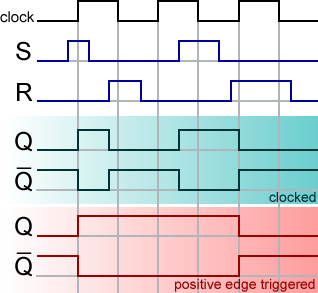
\includegraphics[width=28ex,trim=0 10pt 0 
%     0,clip]{SR_FF_timing_diagram.png}^^A
%   }^^A
%   \def\texta{ (left)}\def\textb{ (right)}^^A
%   }{}^^A
%  \def\exampleextraheader{%
%    \string\let
%    \string\insertoriginalimageforcomparisionifpresent\string\relax
%  }%
% \fi
% \begin{examplecode}
%   \definecolor{bgblue}{rgb}{0.41961,0.80784,0.80784}
%   \definecolor{bgred}{rgb}{1,0.61569,0.61569}
%   \definecolor{fgblue}{rgb}{0,0,0.6}
%   \definecolor{fgred}{rgb}{0.6,0,0}
%   \begin{tikztimingtable}[timing/slope=0,
%     timing/coldist=2pt,xscale=2,yscale=1.1,semithick]
%     \scriptsize clock & 7{C}\\
%     S & .75L h 2.25L H LLl [fgblue]\\
%     R & 1.8L .8H 2.2L 1.4H 0.8L [fgblue]\\
%     Q & L .8H 1.7L 1.5H LL\\
%     $\overline{\mbox{Q}}$ & H .8L 1.7H 1.5L HH\\
%     Q & LHHHHLL[fgred]\\
%     $\overline{\mbox{Q}}$ & HLLLLHH[fgred]\\
%   \extracode
%    \begin{pgfonlayer}{background}
%     \shade [right color=bgblue,left color=white]
%        (7,-8.45) rectangle (-2,-4.6);
%     \shade [right color=bgred,left color=white]
%        (7,-12.8) rectangle (-2,-8.6);
%     \begin{scope}[gray,semitransparent,semithick]
%       \horlines{}
%       \foreach \x in {1,...,6}
%         \draw (\x,1) -- (\x,-12.8);
%       % similar: \vertlines{1,...,6}
%     \end{scope}
%     \node [anchor=south east,inner sep=0pt]
%       at (7,-8.45) {\tiny clocked};
%     \node [anchor=south east,inner sep=0pt,fgred]
%       at (7,-12.8) {\tiny positive edge triggered};
%    \end{pgfonlayer}
%   \end{tikztimingtable}
%   \insertoriginalimageforcomparisionifpresent
% \end{examplecode}
% \caption[SR flip-flop timing diagram]{SR flip-flop timing diagram\texta.  
% Redrawn from image\textb\\ {\small
% \url{http://commons.wikimedia.org/wiki/File:SR_FF_timing_diagram.png}
% }}
% \end{example}
%
% \begin{example}
% \centering
% \lstset{basicstyle=\ttfamily\footnotesize}
% \def\texta{}\def\textb{}^^A
% \begin{examplecode}
%   \newcounter{countup}
%   \newcommand*{\countup}{\addtocounter{countup}{1}\thecountup}
%   \newcommand*{\crst}{\setcounter{countup}{0}}
%   \begin{tikztimingtable}
%     [timing/d/background/.style={fill=white},
%      timing/lslope=0.2]
%             CPOL=0 & LL 15{T} LL \\
%             CPOL=1 & HH 15{T} HH \\
%                    & H 17L H     \\
%     \\
%     \crst Cycle \# & U     8{2D{\countup}} 2U    \\
%     \crst     MISO & D{z}  8{2D{\countup}} 2D{z} \\
%     \crst     MOSI & D{z}  8{2D{\countup}} 2D{z} \\
%     \\
%     \crst Cycle \# & UU    8{2D{\countup}}  U    \\
%     \crst     MISO & D{z}U 8{2D{\countup}}  D{z} \\
%     \crst     MOSI & D{z}U 8{2D{\countup}}  D{z} \\
%   \extracode
%     \begin{pgfonlayer}{background}
%       \begin{scope}[semitransparent,semithick]
%         \vertlines[red]{2.1,4.1,...,17.1}
%         \vertlines[blue]{3.1,5.1,...,17.1}
%       \end{scope}
%     \end{pgfonlayer}
%     \begin{scope}
%       [font=\sffamily\Large,shift={(-6em,-0.5)},anchor=east]
%       \node at (  0, 0) {SCK};    \node at (  0,-3 ) {SS};
%       \node at (1ex,-9) {CPHA=0}; \node at (1ex,-17) {CPHA=1};
%     \end{scope}
%   \end{tikztimingtable}%
% \end{examplecode}
% \caption[SPI Interface Timing]{SPI Interface Timing\texta.  Redrawn from 
% image\textb\\ {\small
% \url{http://en.wikipedia.org/wiki/File:SPI_timing_diagram.svg}}}
% \end{example}
%
% \StopEventually{}
% \FloatBarrier
% \clearpage
% \section{Implementation}
% \subsection{Package Header}
%    \begin{macrocode}
%<*package>
\RequirePackage{tikz}
\usetikzlibrary{calc}
\usetikzlibrary{backgrounds}

\def\tikztimingwidth{0.0}
\newcount\tikztiming@numint
\newcount\tikztiming@numfrac
\def\tikztiming@num{1.0}%
%%\def\tikztiming@num{\the\tikztiming@numint.\the\tikztiming@numfrac}

\newcounter{tikztiming@nrows}%
\def\tikztiming@rowdist{2}%
\def\tikztiming@coldist{1}%
\def\tikztiminglabel#1{#1}%

\def\tikztiming@prefix{tikztiming@trans@}
%    \end{macrocode}

% \subsection{TikZ Style Settings}
%    \begin{macrocode}
\tikzset{timing/.style={%
    x=1.6ex, y=1.6ex,
    line cap=round, line join=round,
  }%
}
\tikzset{%
  timing/.cd,
  grid/.style={timing,help lines},
  intext/.style={timing,line width=0.15ex},
  table/.style={timing,line width=0.15ex,font=\sffamily},
  coord/.style={inner sep=0pt,outer sep=0pt},
  save/.style={inner sep=0pt,outer sep=0pt,/utils/exec=\tikztiming@savesettings},
  restore/.style={/utils/exec=\tikztiming@restoresettings},
  name/.style={inner sep=0pt,outer sep=0pt},
  d/text/.style={timing,scale=0.6,font=\sffamily},
  d/background/.style={},
  h/.style={},
  l/.style={},
  d/.style={},
  m/.style={black!40!brown},
  u/background/.style={fill=gray},
  u/.style={},
  o/background/.style={},
  o/.style={timing/d,line width=0.10ex,dotted},
  z/.style={blue},
  t/.style={},
  c/.style={timing/slope=0.0},
  x/.style={red},
  table/grid/.style={timing/grid},
  table/lines/.style={},
  slope/.code={%
    \tikztimingsetslope{#1}%
    \tikztimingsetdslope{2*#1}%
    \tikztimingsetzslope{#1/2}%
  },
  lslope/.code={\tikztimingsetslope{#1}},
  dslope/.code={\tikztimingsetdslope{#1}},
  zslope/.code={\tikztimingsetzslope{#1}},
  coldist/.store in=\tikztiming@coldist,
  rowdist/.store in=\tikztiming@rowdist,
}
%    \end{macrocode}
%
% \subsection{Macros}
% \begin{macro}{\texttimingbefore}
% This macro is executed inside the tikzpicture environment of \cs{texttiming} 
% before the timing diagram is drawn.
%    \begin{macrocode}
\def\texttimingbefore{}
%    \end{macrocode}
% \end{macro}
%
% \begin{macro}{\texttimingafter}
% This macro is executed inside the tikzpicture environment of \cs{texttiming} 
% after the timing diagram is drawn.
%    \begin{macrocode}
\def\texttimingafter{}
%    \end{macrocode}
% \end{macro}
%
% \begin{macro}{\texttiminggrid}
% Draws a background grid with the `timing/grid' setting. Should be used inside 
% \cs{texttimingbefore}.
%    \begin{macrocode}
\def\texttiminggrid{%
  \draw[xstep={\timingwidth/2.},ystep={\timingheight/2.},timing/grid] (0,0) grid 
  (\timingwidth*\tikztimingwidth,\timingheight);
}
%    \end{macrocode}
% \end{macro}
%
% \begin{macro}{\texttiming}
%    \begin{macrocode}
\DeclareRobustCommand*\texttiming[2][]{%
  \begingroup
    \tikztiming@init
    \uppercase{\def\lastchar{#1}}%
    \@ifundefined{tikztiming@initcode@\lastchar}%
      {}%
      {\@nameuse{tikztiming@initcode@\lastchar}}%
    \ifx\lastchar\empty\else
    \@ifundefined{\tikztiming@prefix\lastchar @start}%
      {\PackageWarning{tikz-timing}{Start value for timing character '\lastchar' 
      is not defined and will be ignored!}{}{}{}}%
      {\tikztiming@nameaddtostr{\lastchar @start}{}}%
    \fi
    \tikztiming@#2\relax
    %\message{^^J\meaning\tikztiming@str^^J}%
    \begin{tikzpicture}[timing/intext]%
      \path[use as bounding box] (0,0) rectangle 
      (\timingwidth*\tikztimingwidth,\timingheight);%
      \texttimingbefore
      \tikztiming@str;%
      \texttimingafter
    \end{tikzpicture}%
  \endgroup
}
%    \end{macrocode}
% \end{macro}
%
% \begin{macro}{\tikztiming@init}
%    \begin{macrocode}
\def\tikztiming@init{%
    \def\lastchar{}%
    \let\currentchar\empty
    \def\tikztimingwidth{0.0}%
    \setcounter{tikztimingtrans}{-1}%
    \def\tikztiming@str{\draw (0,0) coordinate (timing/start base) }%
}
%    \end{macrocode}
% \end{macro}
%
% \begin{macro}{\timing}
%    \begin{macrocode}
\def\timing{%
  \@ifnextchar{[}%
    {\timing@}%
    {\timing@[]}%
}
%    \end{macrocode}
% \end{macro}
%
% \begin{macro}{\timing@}
%    \begin{macrocode}
\def\timing@[#1]{%
  \@ifnextchar{+}%
    {\timing@@{#1}}%
    {\@ifnextchar(%)
      {\timing@@{#1}}%
      {\timing@@{#1}+(0,0)}%
    }%
}
%    \end{macrocode}
% \end{macro}
%
% \begin{macro}{\timing@@}
%    \begin{macrocode}
\def\timing@@#1#2(#3){%
  \timing@@@{#1}{#2(#3)}%
}
%    \end{macrocode}
% \end{macro}
%
% \begin{macro}{\timing@@@}
%    \begin{macrocode}
\def\timing@@@#1#2#3{%
  \begingroup
    \tikztiming@init
    \@ifnextchar{[}%
      {\timing@@@init}%
      {\timing@@@init[]}%
    #3\relax
    %\message{^^J\meaning\tikztiming@str^^J}%
    \begin{scope}[shift={#2},timing,#1]%
      \tikztiming@str;%
    \end{scope}%
  \endgroup
  \timing@@@end
}
%    \end{macrocode}
% \end{macro}
%
% \begin{macro}{\timing@@@end}
%    \begin{macrocode}
\def\timing@@@end#1;{%
  \ifx;#1;\else
    \PackageError{tikz-package}{Can not parse timing path}{}{}{}%
  \fi
}
%
%    \end{macrocode}
% \end{macro}
%
% \begin{macro}{\timing@@@init}
%    \begin{macrocode}
\def\timing@@@init[#1]{%
  \uppercase{\def\lastchar{#1}}%
  \@ifundefined{tikztiming@initcode@\lastchar}%
    {}%
    {\@nameuse{tikztiming@initcode@\lastchar}}%
  \ifx\lastchar\empty\else
  \@ifundefined{\tikztiming@prefix\lastchar @start}%
    {\PackageWarning{tikz-timing}{Start value for timing character '\lastchar' 
    is not defined and will be ignored!}{}{}{}}%
    {\tikztiming@nameaddtostr{\lastchar @start}{}}%
  \fi
  \tikztiming@
}
%    \end{macrocode}
% \end{macro}
%
%
% \begin{macro}{\tikztiming@trans@}
% The empty transition gets defined to avoid errors if it is used by the generic 
% code, e.g. if a non-combinable character like `C' is the last one.
%    \begin{macrocode}
\let\tikztiming@trans@\@gobble
%    \end{macrocode}
% \end{macro}
%
% \begin{macro}{\tikztiming@aftercode@T}
%    \begin{macrocode}
\def\tikztiming@aftercode@T{%
  \tikztiming@output@flush
}
%    \end{macrocode}
% \end{macro}
%
% \begin{macro}{\tikztiming@aftercode@t}
%    \begin{macrocode}
\def\tikztiming@aftercode@t{%
  \tikztiming@aftercode@T
}
%    \end{macrocode}
% \end{macro}
%
% \begin{macro}{\tikztiming@aftercode@C}
%    \begin{macrocode}
\def\tikztiming@aftercode@C{%
  %\tikztiming@output@flush
}
%    \end{macrocode}
% \end{macro}
%
% \begin{macro}{\tikztiming@aftercode@c}
%    \begin{macrocode}
\def\tikztiming@aftercode@c{%
  \tikztiming@aftercode@C
}
%    \end{macrocode}
% \end{macro}
%
% \begin{macro}{\tikztiming@aftercode@G}
%    \begin{macrocode}
\def\tikztiming@aftercode@G{%
  \let\lastchar\secondlastchar
  \let\tikztimingwidth\lasttikztimingwidth
}
%    \end{macrocode}
% \end{macro}
%
% \begin{macro}{\tikztiming@aftercode@g}
%    \begin{macrocode}
\def\tikztiming@aftercode@g{%
  \let\lastchar\secondlastchar
  \let\tikztimingwidth\lasttikztimingwidth
}
%    \end{macrocode}
% \end{macro}
%
% \begin{macro}{\tikztiming@aftercode@S}
%    \begin{macrocode}
\def\tikztiming@aftercode@S{%
  \let\lastchar\secondlastchar
}
%    \end{macrocode}
% \end{macro}
%
% \begin{macro}{\tikztiming@aftercode@s}
%    \begin{macrocode}
\def\tikztiming@aftercode@s{%
  \let\lastchar\secondlastchar
}
%    \end{macrocode}
% \end{macro}
%
% \begin{macro}{\tikztiming@beforenextcode@D@edge@}
%    \begin{macrocode}
\def\tikztiming@beforenextcode@D@edge@{%
  \if D\currentchar\else
    \if d\currentchar\else
      \def\lastchar{D}%
    \fi
  \fi
}
%    \end{macrocode}
% \end{macro}
%
% \begin{macro}{\tikztiming@beforecode@d@edge@}
%    \begin{macrocode}
\def\tikztiming@beforenextcode@d@edge@{%
  \if D\currentchar\else
    \if d\currentchar\else
      \def\lastchar{D}%
    \fi
  \fi
}
%    \end{macrocode}
% \end{macro}
%
% \begin{macro}{\tikztiming@initcode@D}
%    \begin{macrocode}
\def\tikztiming@initcode@D{%
  \def\lastchar{D@edge@}%
}
%    \end{macrocode}
% \end{macro}
%
% \begin{macro}{\tikztiming@initcode@d}
%    \begin{macrocode}
\def\tikztiming@initcode@d{%
  \def\lastchar{d@edge@}%
}
%    \end{macrocode}
% \end{macro}
%
% \begin{macro}{\tikztiming@}
% The |\@ifnextchar\bgroup| is a trick to remove following spaces which would 
% break the number test.
%    \begin{macrocode}
\def\tikztiming@{%
  \@ifnextchar\bgroup
    {\tikztiming@testfornum}%
    {\tikztiming@testfornum}%
}
%    \end{macrocode}
% \end{macro}
%
% \begin{macro}{\tikztiming@eaddtostr}
%    \begin{macrocode}
\def\tikztiming@eaddtostr#1{%
  \begingroup
    \tikztiming@internaldefs{}%
    \@temptokena\expandafter{\tikztiming@str}%
    \xdef\tikztiming@str{%
      \the\@temptokena
      #1%
    }%
  \endgroup
}
%    \end{macrocode}
% \end{macro}
%
% \begin{macro}{\tikztiming@addtostr}
%    \begin{macrocode}
\def\tikztiming@addtostr{%
  \g@addto@macro\tikztiming@str
}
%    \end{macrocode}
% \end{macro}
%
% \begin{macro}{\tikztiming@output}
%    \begin{macrocode}
\def\tikztiming@output#1#2{%
  \ifx\relax#2\relax
    \tikztiming@nameaddtostr{#1}%
  \else
    \ifcase0%
      \ifx\tikztiming@output@bufchara\empty
        \ifx\tikztiming@output@bufcharb\empty
          1%
        \fi
      \fi\relax
      % not empty
      \edef\tikztiming@output@currentchar{#2}%
      \ifcase0%
      \expandafter\ifx\csname tikztiming@nocombine@#2\endcsname\relax
      \ifx\tikztiming@output@currentchar\tikztiming@output@bufcharb
        1%
      \fi\fi
      \relax
        \tikztiming@output@flush
        \edef\tikztiming@output@bufchara{#1}%
        \edef\tikztiming@output@bufcharb{#2}%
      \or
        \pgfmathparse{\tikztiming@output@bufnum + \tikztiming@num}%
        \let\tikztiming@output@bufnum\pgfmathresult
        \def\tikztiming@num{1.0}%
      \fi
    \else % empty
      \edef\tikztiming@output@bufchara{#1}%
      \edef\tikztiming@output@bufcharb{#2}%
      \let\tikztiming@output@bufnum\tikztiming@num
      \def\tikztiming@num{1.0}%
    \fi
  \fi
}
%    \end{macrocode}
%
% Init buffer macros:
%    \begin{macrocode}
\def\tikztiming@output@bufchara{}%
\def\tikztiming@output@bufcharb{}%
\def\tikztiming@output@bufnum{0}%
%    \end{macrocode}
% \end{macro}
%
% \begin{macro}{\tikztiming@output@flush}
%    \begin{macrocode}
\def\tikztiming@output@flush{%
  \begingroup
    \let\tikztiming@num\tikztiming@output@bufnum
    \tikztiming@nameaddtostr{%
      \tikztiming@output@bufchara
      \tikztiming@output@bufcharb
    }%
  \endgroup%
  \gdef\tikztiming@output@bufchara{}%
  \gdef\tikztiming@output@bufcharb{}%
  \global\let\tikztiming@output@bufnum\tikztiming@num
  \gdef\tikztiming@num{1.0}%
}
%    \end{macrocode}
% \end{macro}
%
% \begin{macro}{\tikztiming@nameaddtostr}
%    \begin{macrocode}
\def\tikztiming@nameaddtostr#1{%
  \begingroup
    \edef\@tempa{\tikztiming@num}%
    \expandafter\g@addto@macro
    \expandafter\tikztiming@str
    \expandafter{\csname\tikztiming@prefix#1\expandafter\endcsname
    \expandafter{\@tempa} }%
  \endgroup
  \def\tikztiming@num{1.0}%
}
%    \end{macrocode}
% \end{macro}
%
% \begin{macro}{\tikztiming@nameedef}
%    \begin{macrocode}
\newcommand\tikztiming@nameedef[3][A]{%
  \def\@gtempa##1{#3}%
  \expandafter\let\csname\tikztiming@prefix#2@general\endcsname\@gtempa
  \begingroup
    \tikztiming@internaldefs{#1}%
    \xdef\@gtempa##1{\@gtempa{\width}}%
  \endgroup
  \expandafter\let\csname\tikztiming@prefix#2\endcsname\@gtempa
  \let\@gtempa\empty
}
%    \end{macrocode}
% \end{macro}
%
% \begin{macro}{\tikztiming@namelet}
% Only execute |\let| if the original macro is defined or the destination macro 
% is defined and would now set to undefined.
%    \begin{macrocode}
\newcommand\tikztiming@namelet[2]{%
  \ifcase0%
    \@ifundefined{\tikztiming@prefix#2}%
      {\@ifundefined{\tikztiming@prefix#1}%
        {0}{1}%
      }%
      {1}%
    \relax
  \else
    \expandafter\let
    \csname\tikztiming@prefix#1\expandafter\endcsname
    \csname\tikztiming@prefix#2\endcsname
  \fi
}
%    \end{macrocode}
% \end{macro}
%
% \begin{macro}{\tikztiming@@end}
%    \begin{macrocode}
\def\tikztiming@@end{%
  \tikztiming@output@flush
  \tikztiming@addtostr{ coordinate (timing/end)
    let \p1 = (timing/start base), \p2 = (timing/end) in
      coordinate (timing/end base) at (\x2,\y1)
      coordinate (timing/end top)  at (\x2,1+\y1)
  }%
}
%    \end{macrocode}
% \end{macro}
%
% \begin{macro}{\tikztiming@@}
%    \begin{macrocode}
\def\tikztiming@@#1{%
  \ifx\relax#1\empty
    \expandafter\tikztiming@@end
  \else
    \let\lasttikztimingwidth\tikztimingwidth
    \tikztiming@iflower{#1}%
      {\pgfmathparse{\tikztiming@num/2.0}\let\tikztiming@num\pgfmathresult}%
      {}%
    \pgfmathparse{\tikztimingwidth + \tikztiming@num}%
    \let\tikztimingwidth\pgfmathresult
    \def\currentchar{#1}%
    \uppercase{\def\currentcharuc{#1}}%
    \@ifundefined{tikztiming@beforenextcode@\lastchar}%
      {}%
      {\@nameuse{tikztiming@beforenextcode@\lastchar}}%
    \@ifundefined{tikztiming@beforecode@\currentchar}%
      {}%
      {\@nameuse{tikztiming@beforecode@\currentchar}}%
    \@ifundefined{\tikztiming@prefix\lastchar\currentchar}%
      {\@ifundefined{\tikztiming@prefix\lastchar\currentcharuc}%
        {\PackageWarning{tikz-timing}{Timing transition '\lastchar\currentchar' 
        is not defined and will be ignored!}{}{}{}}%
        {\tikztiming@output{\lastchar}{\currentcharuc}}%
      }%
      {\tikztiming@output{\lastchar}{\currentchar}}%
    \let\secondlastchar\lastchar
    \let\lastchar\currentcharuc
    \@ifundefined{tikztiming@aftercode@\currentcharuc}%
      {}%
      {\@nameuse{tikztiming@aftercode@\currentcharuc}}%
    \expandafter
    \tikztiming@testfortext
  \fi
}
%    \end{macrocode}
% \end{macro}
%
% \begin{macro}{\tikztiming@testfortext}
%    \begin{macrocode}
\def\tikztiming@testfortext{%
  \@ifnextchar\bgroup
    {\tikztiming@handletext}%
    {\tikztiming@}%
}
%    \end{macrocode}
% \end{macro}
%
% \begin{macro}{\tikztiming@handletext}
%    \begin{macrocode}
\def\tikztiming@handletext#1{%
  \@ifnextchar{[}%
    {\tikztiming@handletext@}%
    {\tikztiming@handletext@[]}%
  #1\relax
}
%    \end{macrocode}
% \end{macro}
%
% \begin{macro}{\tikztiming@handletext@}
%    \begin{macrocode}
\def\tikztiming@handletext@[#1]#2\relax{%
  \begingroup
  \expandafter\lowercase\expandafter{%
    \expandafter\def\expandafter\currentcharlc
    \expandafter{\currentchar}%
  }%
  \pgfkeysifdefined{/tikz/timing/\currentcharlc/text/.@cmd}%
  {%
  \tikztiming@output@flush
  \tikztiming@eaddtostr{%
    node (timing@dend) at +(\dslope/2.0,\height/2.0) {}
    node [%]
      shift={($ (timing@dstart)!0.5!(timing@dend) $)},%
      timing/\currentcharlc/text,%
  }%
  \endgroup
  \tikztiming@addtostr{%[
      #1%
      ] {#2}%
  }%
  \def\lastchar{D@edge@}%
  }{%
    \endgroup
    \PackageWarning{tikz-timing}{Ignoring text for character 
    '\currentchar'!}{}{}{}%
  }%
  \tikztiming@
}
%    \end{macrocode}
% \end{macro}
%
% \begin{macro}{\tikztiming@stoppath}
%    \begin{macrocode}
\def\tikztiming@stoppath#1{%
  \tikztiming@output@flush
  \tikztiming@eaddtostr{%
    \newdraw
  }%
  \tikztiming@
}
%    \end{macrocode}
% \end{macro}
%
% \begin{macro}{\tikztiming@stoppath@nosave}
%    \begin{macrocode}
\def\tikztiming@stoppath@nosave#1{%
  \tikztiming@output@flush
  \tikztiming@eaddtostr{%
    \newdrawns
  }%
  \tikztiming@
}
%    \end{macrocode}
% \end{macro}
%
%
% \begin{macro}{\tikztiming@testforcode}
%    \begin{macrocode}
\def\tikztiming@testforcode{%
  \@ifnextchar{!}%
    {\tikztiming@testforcode@}%
    {\@ifnextchar{[}%
      {\tikztiming@handleoption}%
      {\@ifnextchar{;}%
        {\tikztiming@stoppath@nosave}%
        {\@ifnextchar{,}%
          {\tikztiming@stoppath}%
          {\tikztiming@@}%
        }%
      }%
    }%
}
%    \end{macrocode}
% \end{macro}
%
% \begin{macro}{\tikztiming@testforcode@}
%    \begin{macrocode}
\def\tikztiming@testforcode@#1{%
  \@ifnextchar\bgroup
    {\tikztiming@handlecode}%
    {%
      \PackageWarning{tikz-timing}{Missing braces after '!' character. Ignoring 
      this character}{}{}{}%
      \tikztiming@
    }%
}
%    \end{macrocode}
% \end{macro}
%
% \begin{macro}{\tikztiming@handlecode}
%    \begin{macrocode}
\def\tikztiming@handlecode#1{%
  \tikztiming@output@flush
  \tikztiming@addtostr{ #1 }%
  \tikztiming@
}
%    \end{macrocode}
% \end{macro}
%
% \begin{macro}{\tikztiming@handleoption}
%    \begin{macrocode}
\def\tikztiming@handleoption[#1]{%
  \tikztiming@addtostr{ [#1] }%
  \tikztiming@
}
%    \end{macrocode}
% \end{macro}
%

% \begin{macro}{\tikztiming@testfornum}
%    \begin{macrocode}
\def\tikztiming@testfornum{%
  \let\tikztiming@numchars\empty
  \tikztiming@numfrac0\relax
  \afterassignment
  \tikztiming@testfornum@
  \tikztiming@numint0%
}
%    \end{macrocode}
% \end{macro}
%
% \begin{macro}{\tikztiming@testfornumfrac}
%    \begin{macrocode}
\def\tikztiming@testfornumfrac{%
  \afterassignment
  \tikztiming@testfornum@@@
  \tikztiming@numfrac1%
}
%    \end{macrocode}
% \end{macro}
%
% \begin{macro}{\tikztiming@numloop}
%    \begin{macrocode}
\def\tikztiming@numloop{%
  \ifnum\tikztiming@numint>0%
    \toks@\expandafter{\tikztiming@numchars}%
    \xdef\tikztiming@numchars{%
      \the\toks@
      \the\@temptokena
    }%
    \advance\tikztiming@numint by -1\relax
    \expandafter\tikztiming@numloop
  \fi
}
%    \end{macrocode}
% \end{macro}
%
% \begin{macro}{\tikztiming@testfornum@}
%    \begin{macrocode}
\def\tikztiming@testfornum@{%
  \ifnum0<\tikztiming@numint
    \let\tikztiming@next\tikztiming@testfornum@@
  \else
    \def\tikztiming@next{%
      \@ifnextchar{.}%
        {\expandafter\tikztiming@testfornumfrac\@gobble}%
        {%
          \tikztiming@numint1\relax
          \tikztiming@numfrac0\relax
          \def\tikztiming@num{1.0}%
          \expandafter\tikztiming@testforcode
        }%
    }%
  \fi
  \tikztiming@next
}
%    \end{macrocode}
% \end{macro}
%
% \begin{macro}{\tikztiming@testfornum@@}
%    \begin{macrocode}
\def\tikztiming@testfornum@@{%
  \@ifnextchar{.}%
    {\expandafter\tikztiming@testfornumfrac\@gobble}%
    {\tikztiming@testfornum@@@}%
}
%    \end{macrocode}
% \end{macro}
%
% \begin{macro}{\tikztiming@testfornum@@@}
%    \begin{macrocode}
\def\tikztiming@testfornum@@@{%
  \xdef\tikztiming@num{\the\tikztiming@numint.\expandafter\@gobble\the\tikztiming@numfrac}%
  \@ifnextchar\bgroup
    {%
      \expandafter\tikztiming@numfrac\expandafter0\expandafter
      \@gobble\the\tikztiming@numfrac\relax
      \ifnum0=\tikztiming@numfrac\else
        \pgfmathparse{round(\tikztiming@num)}%
        \PackageWarning{tikz-timing}%
          {Can not repeat group by a non-integer factor!^^J%
           Rounding '\tikztiming@num' to '\pgfmathresult'.}{}{}{}%
        \let\tikztiming@num\pgfmathresult
      \fi
      \tikztiming@testfornum@@@@
    }%
    {%
      \tikztiming@testforcode
    }%
}
%    \end{macrocode}
% \end{macro}
%
% \begin{macro}{\tikztiming@testfornum@@@@}
%    \begin{macrocode}
\def\tikztiming@testfornum@@@@#1{%
  \begingroup
    \@temptokena{#1}%
    \tikztiming@numloop%
  \endgroup
  \tikztiming@numint1\relax
  \tikztiming@numfrac0\relax
  \expandafter\tikztiming@\tikztiming@numchars
}
%    \end{macrocode}
% \end{macro}
%
% \subsection{Table environment}
%    \begin{macrocode}
%\usetikzlibrary{backgrounds}
\RequirePackage{environ}
\newcounter{tikztimingrows}
%    \end{macrocode}
%
% \begin{macro}{\tikztiming@extracode}
%    \begin{macrocode}
\def\tikztiming@extracode{\@gobble{EXTRACODE}}%
%    \end{macrocode}
% \end{macro}

% \begin{environment}{tikztimingtable}
%    \begin{macrocode}
\NewEnviron{tikztimingtable}[1][]{%
  \begingroup
  \setcounter{tikztiming@nrows}{0}%
  \let\extracode\tikztiming@extracode
  \let\tablegrid\tikztiming@tablegrid
  \let\horlines\tikztiming@horlines
  \let\vertlines\tikztiming@vertlines
  \let\fulltablegrid\tikztiming@fulltablegrid
  \def\rowdist{\tikztiming@rowdist}%
  \def\coldist{\tikztiming@coldist}%
  \def\nrows{\the\c@tikztiming@nrows}%
  \begin{tikzpicture}[timing/table,#1]%
    \coordinate (last row)  at (0,\rowdist);
    \coordinate (label pos) at (-1*\coldist,0);
    \coordinate (timing/table/top left) at (0,1);
    \coordinate (timing/table/bottom right) at (0,0);
    \expandafter\tikztimingtable@row\BODY\endtikztimingtable@
  \end{tikzpicture}
  \endgroup
}

\def\endtikztimingtable@{\@gobble{ENDTIKSTIMING}}
%    \end{macrocode}
% \end{environment}

% \begin{macro}{\tikztimingextracode}
%    \begin{macrocode}
\long\def\tikztimingextracode#1#2\endtikztimingtable@{%
  \path let
     \p1 = (timing/table/top left),
     \p2 = (timing/table/bottom right)
   in
     coordinate (timing/table/bottom left) at (\x1,\y2)
     coordinate (timing/table/top right) at (\x2,\y1)
     coordinate (timing/table/size) at (\x2-\x1,\y1-\y2)
   ;
  #2%
}
%    \end{macrocode}
% \end{macro}
%
% \begin{macro}{\tikztiming@emptycell}
% Just used as marker. Needs unique definition.
%    \begin{macrocode}
\def\tikztiming@emptycell{%
  \@gobble{tikztiming@emptycell}%
}
%    \end{macrocode}
% \end{macro}
%
% \begin{macro}{\tikztimingtable@row}
%    \begin{macrocode}
\def\tikztimingtable@row#1\\{%
  \tikztimingtable@row@#1&\tikztiming@emptycell&\\
}
%    \end{macrocode}
% \end{macro}
%
% \begin{macro}{\tikztimingtable@row@}
%    \begin{macrocode}
\def\tikztimingtable@row@#1&#2&#3\\{%
  \ifx\\#3\\\else
    \begingroup
      \def\@tempa{\tikztiming@emptycell&}%
      \def\@tempb{#3}%
      \ifx\@tempa\@tempb\else
        \PackageWarning{tikz-timing}{%
          To many columns in tikztimingtable row! Only two are allowed%
        }{}{}{}%
      \fi
    \endgroup
  \fi
  \ifx\tikztiming@emptycell#2%
    \def\next{\tikztimingtable@row@@{#1}{}}%
  \else
    \def\next{\tikztimingtable@row@@{#1}{#2}}%
  \fi
  \next
}%
%    \end{macrocode}
% \end{macro}
%
% \begin{macro}{\tikztimingtable@row@@}
%    \begin{macrocode}
\def\tikztimingtable@row@@#1#2{%
  \addtocounter{tikztiming@nrows}{1}%
  \path (last row) +(0,-1*\rowdist) coordinate (last row);
  \path (last row) +(-1*\coldist,0) node [anchor=base east,timing/name]
    {\tikztiminglabel{#1}};
  \timing (last row) {#2};
  \path let \p1 = (timing/table/bottom right), \p2 = (timing/end base) in
    coordinate (timing/table/bottom right) at ({max(\x1,\x2)},\y2);
  \@ifnextchar\extracode
    {%
      \let\extracode\relax
      \tikztimingextracode
    }%
    {%
      \@ifnextchar\endtikztimingtable@
        {\@gobble}{\tikztimingtable@row}%
    }%
}
%    \end{macrocode}
% \end{macro}

% \begin{macro}{\tikztiming@fulltablegrid}
%    \begin{macrocode}
\newcommand*\tikztiming@fulltablegrid[1][]{%
  \begin{pgfonlayer}{background}
    \scope[xstep={\timingwidth/2.},ystep={\timingheight/2.},
    shift={(timing/table/bottom left)},timing/table/grid,#1]
      \draw (0,0) grid
        ($ (timing/table/top right) - (timing/table/bottom left) $);
   \endscope
  \end{pgfonlayer}
}
%    \end{macrocode}
% \end{macro}
%
% \begin{macro}{\tikztiming@tablegrid}
%    \begin{macrocode}
\newcommand*\tikztiming@tablegrid[1][]{%
  \begin{pgfonlayer}{background}
    \scope[xstep={\timingwidth/2.},ystep={\timingheight/2.},timing/table/grid,#1]
      \foreach \y in {1,...,\nrows} {%
        \draw {[shift={($ (timing/table/bottom left) + (0,\y*\rowdist) - 
        (0,\rowdist) $)}] let \p1 = (timing/table/bottom right) in (0,0) grid 
        (\x1,1)};
      }%
    \endscope
  \end{pgfonlayer}
}
%    \end{macrocode}
% \end{macro}
%
% \begin{macro}{\tikztiming@horlines}
%    \begin{macrocode}
\newcommand*\tikztiming@horlines[2][]{%
  \begingroup
    \def\list{#2}%
    \ifx\list\empty
      \def\list{1,2,...,\nrows}%
    \fi
    \foreach \row in \list%
      \draw [timing/table/lines,#1] let
        \p1 = (timing/table/bottom right)
      in
        (0,\rowdist-\row*\rowdist) -- +(\x1,0);
  \endgroup
}
%    \end{macrocode}
% \end{macro}
%
% \begin{macro}{\tikztiming@vertlines}
%    \begin{macrocode}
\newcommand*\tikztiming@vertlines[2][]{%
  \begingroup
    \def\list{#2}%
    \ifx\list\empty
      \def\list{0,1,...,16383}%
    \fi
      \draw [timing/table/lines,#1] let
        \p1 = ($ (timing/table/bottom right) - (0,2) $),
        \p2 = (1,0)
      in
        \foreach \clk in \list {
          (\clk,+1.5) -- +(0,\y1-\y2)
          [/utils/exec={\pgfmathparse{\x1>\clk*\x2}%
          \ifnum0=\pgfmathresult
            \breakforeach
            \fi}]
        }
      ;
  \endgroup
}
%    \end{macrocode}
% \end{macro}
%
% \subsection{Other Macros}
%
% \begin{macro}{\tikztiming@iflower}
%    \begin{macrocode}
\def\tikztiming@iflower#1{%
  \begingroup
  \edef\@tempa{`#1}%
  \ifnum\@tempa=\lccode\@tempa
    \endgroup
    \expandafter
    \@firstoftwo
  \else
    \endgroup
    \expandafter
    \@secondoftwo
  \fi
}
%    \end{macrocode}
% \end{macro}
%
% \begin{macro}{\timingwidth}
% \begin{macro}{\timingheight}
%    \begin{macrocode}
\def\timingwidth{1}%
\def\timingheight{1}%
%    \end{macrocode}
% \end{macro}
% \end{macro}
%
% \begin{macro}{\tikztiming@internaldefs}
%    \begin{macrocode}
\def\tikztiming@internaldefs#1{%
  \def\draw{\noexpand\draw}%
  \def\path{\noexpand\path}%
  \def\fill{\noexpand\fill}%
  \def\width{####1*\noexpand\timingwidth}%
  \def\fwidth{\noexpand\timingwidth}%
  \def\height{\noexpand\timingheight}%
  \def\slope{\noexpand\timingslope}%
  \def\zslope{\noexpand\timingzslope}%
  \def\dslope{\noexpand\timingdslope}%
  \def\gslope{0}%
  \lowercase{%
  \def\style{timing/#1}%
  \def\bgstyle{timing/#1/background}%
  }%
  \def\newdraw{\tikztiming@newdraw}%
  \def\newdrawns{\tikztiming@newdraw@nosave}%
  \def\code##1{ [/utils/exec={\unexpanded{##1}}] }%
}
%    \end{macrocode}
% \end{macro}

% \begin{macro}{\tikztimingsetslope}
%    \begin{macrocode}
\def\tikztimingsetslope#1{%
  \pgfmathparse{min(1.0,{max(0.0,#1)})}%
  \let\tikztiming@slope\pgfmathresult
  \edef\timingslope{\tikztiming@slope*\noexpand\timingwidth}%
}
%    \end{macrocode}
% \end{macro}
%
% \begin{macro}{\tikztimingsetdslope}
%    \begin{macrocode}
\def\tikztimingsetdslope#1{%
  \pgfmathparse{min(1.0,{max(0.0,#1)})}%
  \let\tikztiming@dslope\pgfmathresult
  \edef\timingdslope{\tikztiming@dslope*\noexpand\timingwidth}%
}
%    \end{macrocode}
% \end{macro}
%
% \begin{macro}{\tikztimingsetzslope}
%    \begin{macrocode}
\def\tikztimingsetzslope#1{%
  \pgfmathparse{min(1.0,{max(0.0,#1)})}%
  \let\tikztiming@zslope\pgfmathresult
  \edef\timingzslope{\tikztiming@zslope*\noexpand\timingwidth}%
}
%    \end{macrocode}
% \end{macro}
%    \begin{macrocode}
\tikztimingsetslope{0.10}%
\tikztimingsetdslope{0.20}%
\tikztimingsetzslope{0.05}%
%    \end{macrocode}
%
% \begin{macro}{\tikztiminguse}
%    \begin{macrocode}
\def\tikztiminguse#1{%
  \@ifundefined{\tikztiming@prefix#1@general}%
    {\PackageWarning{Can not use transition macro for '#1'.}{}{}{}}%
    {\@nameuse{\tikztiming@prefix#1@general}}%
}
%    \end{macrocode}
% \end{macro}
%
% \begin{macro}{\tikztimingdef}
%    \begin{macrocode}
\def\tikztimingdef#1{%
  \tikztimingdef@#1\relax%
}
%    \end{macrocode}
% \end{macro}
%
% \begin{macro}{\tikztimingdef@}
%    \begin{macrocode}
\def\tikztimingdef@#1#2\relax#3{%
  \ifx\relax#2\relax
    \tikztiming@nameedef[#1]{#1}{#3}%
  \else
    \tikztiming@nameedef[#2]{#1#2}{#3}%
  \fi
}
%    \end{macrocode}
% \end{macro}
%
% \begin{macro}{\tikztiminglet}
%    \begin{macrocode}
\def\tikztiminglet#1#2{%
  \tikztiminglet@#1\relax#2\relax
}
%    \end{macrocode}
% \end{macro}
%
% \begin{macro}{\tikztiminglet@}
%    \begin{macrocode}
\def\tikztiminglet@#1#2\relax#3#4\relax{%
  \tikztiming@namelet{#1#2}{#3#4}%
  \tikztiming@namelet{#1#2@general}{#3#4@general}%
  \tikztiming@iflower{#1}{}%
    {\tikztiming@iflower{#2}%
      {%
        \lowercase{\tikztiminglet@{#1}{#2}\relax{#3}{#4}}\relax
      }%
      {%
        \uppercase{\lowercase{%
        \uppercase{\lowercase{\tikztiminglet@{#1}}{#2}}\relax{#3}}{#4}}\relax
        \lowercase{\uppercase{%
        \lowercase{\uppercase{\tikztiminglet@{#1}}{#2}}\relax{#3}}{#4}}\relax
      }%
    }%
}
%    \end{macrocode}
% \end{macro}
%
% \begin{macro}{\tikztiming@chars}
%    \begin{macrocode}
\def\tikztiming@chars#1{}
%    \end{macrocode}
% \end{macro}
%
% \begin{macro}{\tikztiming@ifcharexists}
%    \begin{macrocode}
\def\tikztiming@ifcharexists#1{%
  \def\tikztiming@ifcharexists@##1,#1,##2\relax{%
    \ifx\relax##2\relax%
      \expandafter\@firstoftwo
    \else
      \expandafter\@secondoftwo
    \fi
  }%
  \expandafter\tikztiming@ifcharexists@
  \expandafter,\tikztiming@chars,#1,\relax%
}
%    \end{macrocode}
% \end{macro}
%
%
% \begin{macro}{\tikztiming@addchar}
%    \begin{macrocode}
\def\tikztiming@addchar#1{%
  \tikztiming@ifcharexists{#1}{%
    \edef\tikztiming@chars{\tikztiming@chars,#1}%
  }{}%
}
%    \end{macrocode}
% \end{macro}
%
% \begin{macro}{\tikztimingchar}
%    \begin{macrocode}
\def\tikztimingchar#1{%
  \uppercase{%
  \tikztiming@addchar{#1}%
  \tikztimingchar@{#1}}%
}
%    \end{macrocode}
% \end{macro}
%
%    \begin{macrocode}
\expandafter\def\csname\tikztiming@prefix @start\endcsname#1{}%
%    \end{macrocode}
%
% \begin{macro}{\tikztimingchar@}
%    \begin{macrocode}
\def\tikztimingchar@#1#2#3{%
  \tikztiming@nameedef[#1]{#1@start}{#2 coordinate (timing/start) }%
  \tikztiming@nameedef[#1]{#1}{#2 coordinate (timing/start) #3}%
  \tikztimingdef{#1#1}{#3}%
}
%    \end{macrocode}
% \end{macro}
%
% \begin{macro}{\tikztimingalias}
%    \begin{macrocode}
\def\tikztimingalias#1#2{%
  \uppercase{\tikztimingalias@{#1}{#2}}%
}
%    \end{macrocode}
% \end{macro}
%
% \begin{macro}{\tikztimingalias@}
%    \begin{macrocode}
\def\tikztimingalias@#1#2{%
  \tikztiming@namelet{#1}{#2}%
  \tikztiming@namelet{#1@start}{#2@start}%
  \lowercase{%
  \tikztiming@namelet{#1}{#2}%
  \tikztiming@namelet{#1@start}{#2@start}%
  }%
  \tikztiminglet{#1#1}{#2#2}%
  \@for\@tempa:=\tikztiming@chars\do{%
    \expandafter\tikztiminglet@@
    \expandafter{\@tempa}{#1}{#2}%
  }%
}
%    \end{macrocode}
% \end{macro}
%
% \begin{macro}{\tikztimingecopy}
%    \begin{macrocode}
\def\tikztimingecopy#1#2{%
  \uppercase{\tikztimingecopy@{#1}{#2}}%
}
%    \end{macrocode}
% \end{macro}
%
% \begin{macro}{\tikztimingecopy@}
%    \begin{macrocode}
\def\tikztimingecopy@#1#2{%
  \tikztimingchar{#1}{}{}%
  \tikztimingdef{#1}{\tikztiminguse{#2}{##1}}%
  \tikztiming@nameedef[#1]{#1@start}{\tikztiminguse{#2@start}{##1}}%
  \lowercase{%
    \@ifundefined{\tikztiming@prefix#2}{}{%
      \tikztimingdef{#1}{\tikztiminguse{#2}{##1}}%
      \tikztiming@nameedef[#1]{#1@start}{\tikztiminguse{#2@start}{##1}}%
    }%
  }%
  \tikztimingdef{#1#1}{\tikztiminguse{#2#2}{##1}}%
  \@for\@tempa:=\tikztiming@chars\do{%
    \expandafter\tikztimingdef@@
    \expandafter{\@tempa}{#1}{#2}%
%    \end{macrocode}
%    Handle lowercase macros:
%    \begin{macrocode}
    \expandafter\lowercase\expandafter{\expandafter\def\expandafter\@tempb
    \expandafter{\@tempa}}%
    \@ifundefined{\tikztiming@prefix#2\@tempb}{}{%
      \expandafter\tikztimingdef@@
      \expandafter{\@tempb}{#1}{#2}%
    }%
  }%
}
%    \end{macrocode}
% \end{macro}
%
% \begin{macro}{\tikztiminglet@@}
%    \begin{macrocode}
\def\tikztiminglet@@#1#2#3{%
  \tikztiminglet@@@#1#2#3%
  % Should stay, cause no harm:
  \lowercase{\tikztiminglet@@@#1}#2#3%
  \lowercase{\tikztiminglet@@@#1#2#3}%
  \lowercase{\uppercase{\tikztiminglet@@@#1}#2#3}%
}
%    \end{macrocode}
% \end{macro}
%
% \begin{macro}{\tikztiminglet@@@}
%    \begin{macrocode}
\def\tikztiminglet@@@#1#2#3{%
  \tikztiminglet{#1#2}{#1#3}%
  \tikztiminglet{#2#1}{#3#1}%
}
%    \end{macrocode}
% \end{macro}

%
% \begin{macro}{\tikztimingdef@@}
%    \begin{macrocode}
\def\tikztimingdef@@#1#2#3{%
  \tikztimingdef{#1#2}{\tikztiminguse{#1#3}{##1}}%
  \tikztimingdef{#2#1}{\tikztiminguse{#3#1}{##1}}%
}
%    \end{macrocode}
% \end{macro}
%
% \begin{macro}{\tikztiming@savesettings}
%    \begin{macrocode}
\def\tikztiming@savesettings{%
  \xdef\tikztiming@saved@settings{%
    {\tikztiming@slope}%
    {\tikztiming@dslope}%
    {\tikztiming@zslope}%
    {\the\pgflinewidth}%
  }%
}
%    \end{macrocode}
% \end{macro}
%
% \begin{macro}{\tikztiming@restoresettings}
%    \begin{macrocode}
\def\tikztiming@restoresettings{%
  \expandafter\tikztiming@restoresettings@
  \tikztiming@saved@settings\relax
}
%    \end{macrocode}
% \end{macro}
%
% \begin{macro}{\tikztiming@restoresettings@}
%    \begin{macrocode}
\def\tikztiming@restoresettings@#1#2#3#4\relax{%
  \tikztimingsetslope{#1}%
  \tikztimingsetdslope{#2}%
  \tikztimingsetzslope{#3}%
  \pgfsetlinewidth{#4}%
}
%    \end{macrocode}
% \end{macro}
%
% \begin{macro}{\tikztiming@newdraw}
%    \begin{macrocode}
\def\tikztiming@newdraw{%
  node [timing/save] (timing@save) {};%
  \draw [timing/restore] (timing@save) ++(0,0)
}
%    \end{macrocode}
% \end{macro}

% \begin{macro}{\tikztiming@newdraw}
%    \begin{macrocode}
\def\tikztiming@newdraw@nosave{%
  node [timing/coord] (timing@save) {};%
  \draw (timing@save) ++(0,0)
}
%    \end{macrocode}
% \end{macro}

% \subsection{Definition of Timing Characters}
%    \begin{macrocode}
\tikztimingchar{H}{++(0,\height)}{-- ++(#1,0)}

\tikztimingchar{L}{++(0,0)}{-- ++(#1,0)}

\tikztimingchar{Z}{++(0,\height/2.)}{%
  \newdraw [\style]
  -- ++(#1,0)
}

\tikztimingchar{X}{}{}%
\tikztimingchar{D}{}{}%
\tikztimingchar{U}{}{}%
%\tikztimingchar{O}{}{}%
\tikztimingchar{M}{}{}%

\tikztimingchar{G}{++(0,0)}{-- ++(\gslope,\height) -- ++(\gslope,-\height)}
\tikztimingchar{S}{++(0,0)}{++(#1,0)}

\tikztimingdef{DD}{
  node [timing/save] (timing@save) {}; \path [\bgstyle] (timing@save) ++(0,0)
     +(0.5*\dslope,0.5*\height) -- +(\dslope,0)
  -- +(#1,0)
  -- +($ (#1,0) + 0.5*(\dslope,\height) $)
  -- +(#1,\height)
  -- +(\dslope,\height) -- cycle;
  \draw [timing/restore,\style] (timing@save) ++(0,0)
  node [timing/save] (timing@dstart) at +(\dslope/2.,\height/2.) {}
  --  +(\dslope,+\height) --  +(#1,+\height) ++(0,+\height)
  --  +(\dslope,-\height) -- ++(#1,-\height)
}
\tikztiming@namelet{D@edge@D}{DD}
\tikztiming@namelet{D@edge@D@general}{DD@general}

\tikztimingchar{D}{++(0,0)}{
  node [timing/save] (timing@save) {}; \path [\bgstyle] (timing@save) ++(0,0)
  -- +(#1,0)
  -- +($ (#1,0) + 0.5*(\dslope,\height) $)
  -- +(#1,\height)
  -- +(0,\height)
  -- cycle;
  \draw [timing/restore,\style] (timing@save) ++(0,0)
  node [timing/save] (timing@dstart) at +(-\dslope/2.,\height/2.0) {}
  --  +(#1,0) ++(0,+\height)
  -- ++(#1,0) ++(0,-\height)
}

\tikztimingdef{DD}{
  node [timing/save] (timing@save) {}; \path [\bgstyle] (timing@save) ++(0,0)
  -- +(#1,0)
  -- +($ (#1,0) + 0.5*(\dslope,\height) $)
  -- +(#1,\height)
  -- +(0,\height)
  -- cycle;
  \newdraw [\style]
  --  +(#1,0) ++(0,+\height)
  -- ++(#1,0) ++(0,-\height)
}

\tikztiming@namelet{D@edge@@start}{D@start}
\tikztiming@namelet{d@edge@@start}{d@start}

\def\tikztiming@trans@D@fill#1#2{%
  node [timing/save] (timing@save) {}; \path [\bgstyle] (timing@save) ++(0,0)
  -- +(0.5*\dslope,-0.5*\height)
  -- ++($ (#1,-0.5*\height) - (#2,0) $)
  -- +(0.5*\dslope,0.5*\height)
  -- +(0,\height)
  -- ++($ (#2,\height) - (#1,0) + (0.5*\dslope,0) $)
  -- cycle;
  \draw [timing/restore,\style] (timing@save) ++(0,0)
  node [timing/save] (timing@dstart) {}
}

\tikztimingdef{HH}{-- ++(#1,0)}
\tikztimingdef{LL}{-- ++(#1,0)}
\tikztimingdef{HL}{-- ++(\slope,-\height) \tikztiminguse{HH}{#1-\slope}}
\tikztimingdef{LH}{-- ++(\slope, \height) \tikztiminguse{LL}{#1-\slope}}

\tikztimingdef{HG}{-- ++(\gslope,-\height) -- ++(\gslope,+\height)}
\tikztimingdef{LG}{-- ++(\gslope,+\height) -- ++(\gslope,-\height)}
\tikztimingdef{ZG}{
  -- ++(\gslope,-\height/2.0)
  -- ++(\gslope,+\height)
  -- ++(\gslope,-\height/2.0)
}
\tikztiminglet{DG}{LG}
\tikztiminglet{MG}{ZG}

\tikztiminglet{HS}{S}
\tikztiminglet{LS}{S}
\tikztiminglet{ZS}{S}
\tikztiminglet{DS}{S}
\tikztiminglet{TS}{S}

\tikztimingdef{LZ}{
  \newdraw [\style]
  -- ++(\zslope,+\height/2.) -- ++($ (#1,0) - (\zslope,0) $)
}
\tikztimingdef{HZ}{%
  \newdraw [\style]
  -- ++(\zslope,-\height/2.) -- ++($ (#1,0) - (\zslope,0) $)
}
  \tikztimingdef{ZH}{
    \newdraw
  -- ++(\zslope,+\height/2.) -- ++($ (#1,0) - (\zslope,0) $)
}
\tikztimingdef{ZL}{%
  \newdraw
  -- ++(\zslope,-\height/2.) -- ++($ (#1,0) - (\zslope,0) $)
}

\tikztimingdef{DZ}{
  -- ++( \dslope/2.,+\height/2.)
     ++(-\dslope/2.,+\height/2.)
  -- ++( \dslope/2.,-\height/2.)
  \newdraw [\style]
  -- ++($ (#1,0) - (\dslope/2.,0) $)
}

\tikztimingdef{ZD}{
  \tikztiming@trans@D@fill{#1}{0}%
  -- ++(\dslope/2.,\height/2.)  -- ++($ (#1,0) - (\dslope/2.,0) $)
     ++($ -1*(#1,0) + (0,-\height/2.) $)
  -- ++(\dslope/2.,-\height/2.) -- ++($ (#1,0) - (\dslope/2.,0) $)
}

\tikztimingdef{LD}{
  -- ++(0.5*\dslope,0.5*\height)
  \tikztiming@trans@D@fill{#1}{0.5*\dslope}%
  -- ++(0.5*\dslope,0.5*\height)
  -- ++($ (#1,0) - (\dslope,0) $)
     ++($ -1*(#1,0) + (0,-\height) $)          ++(\dslope/2.,+\height/2.)
  -- ++(\dslope/2.,-\height/2.) -- ++($ (#1,0) - (\dslope,0) $)
}

\tikztimingdef{DL}{
  -- ++( \dslope/2.,+\height/2.)
     ++(-\dslope/2.,+\height/2.)
  -- ++(\dslope/2.,-\height/2.)
  \newdraw [\style]
  -- ++(\dslope/2.,-\height/2.)
  -- ++($ (#1,0) - (\dslope,0) $)
}

\tikztimingdef{HD}{
  -- ++(0.5*\dslope,-0.5*\height)
  \tikztiming@trans@D@fill{#1}{0.5*\dslope}%
  -- ++(0.5*\dslope,-0.5*\height)
  -- ++($ (#1,0) - (\dslope,0) $)
     ++($ -1*(#1,0) + (0,+\height) $)          ++(\dslope/2.,-\height/2.)
  -- ++(\dslope/2.,+\height/2.) -- ++($ (#1,0) - (\dslope,0) $)
     ++(0,-\height)
}

\tikztimingdef{DH}{
     ++(0,+\height)
  -- ++(+\dslope/2.,-\height/2.)
     ++(-\dslope/2.,-\height/2.)
  -- ++(\dslope/2.,+\height/2.)
  \newdraw [\style]
  -- ++(\dslope/2.,+\height/2.)
  -- ++($ (#1,0) - (\dslope,0) $)
}


\tikztimingalias{M}{Z}
\tikztimingchar{M}{++(0,\height/2.)}{
  [\style]
  -- ++($ 1/16.*(#1,0) + (0,+\height*.225) $)
  -- ++($ 1/8.*(#1,0) + (0,-\height*.45) $)
  -- ++($ 1/8.*(#1,0) + (0,+\height*.45) $)
  -- ++($ 1/8.*(#1,0) + (0,-\height*.45) $)
  -- ++($ 1/8.*(#1,0) + (0,+\height*.45) $)
  -- ++($ 1/8.*(#1,0) + (0,-\height*.45) $)
  -- ++($ 1/8.*(#1,0) + (0,+\height*.45) $)
  -- ++($ 1/8.*(#1,0) + (0,-\height*.45) $)
  -- ++($ 1/16.*(#1,0) + (0,+\height*.225) $)
}

\tikztimingdef{MZ}{
  \newdraw [\style]
  -- ++(#1,0)
}

\tikztimingdef{m}{
  [\style]
     ++(0,+\height/2.)
  -- ++($ 1/8.*(#1,0) + (0,+\height*.225) $)
  -- ++($ 1/4.*(#1,0) + (0,-\height*.45) $)
  -- ++($ 1/4.*(#1,0) + (0,+\height*.45) $)
  -- ++($ 1/4.*(#1,0) + (0,-\height*.45) $)
  -- ++($ 1/8.*(#1,0) + (0,+\height*.225) $)
}

\tikztimingdef{ZM}{
  \newdraw [\style]
  -- ++($ 1/16.*(#1,0) + (0,+\height*.075) $)
  -- ++($ 1/8.*(#1,0) + (0,-\height*.20) $)
  -- ++($ 1/8.*(#1,0) + (0,+\height*.25) $)
  -- ++($ 1/8.*(#1,0) + (0,-\height*.30) $)
  -- ++($ 1/8.*(#1,0) + (0,+\height*.35) $)
  -- ++($ 1/8.*(#1,0) + (0,-\height*.40) $)
  -- ++($ 1/8.*(#1,0) + (0,+\height*.45) $)
  -- ++($ 1/8.*(#1,0) + (0,-\height*.45) $)
  -- ++($ 1/16.*(#1,0) + (0,+\height*.225) $)
}

\tikztimingdef{Zm}{
  \newdraw [\style]
  -- ++($ 1/8.*(#1,0) + (0,+\height*.075) $)
  -- ++($ 1/4.*(#1,0) + (0,-\height*.20) $)
  -- ++($ 1/4.*(#1,0) + (0,+\height*.25) $)
  -- ++($ 1/4.*(#1,0) + (0,-\height*.30) $)
  -- ++($ 1/8.*(#1,0) + (0,+\height*.175) $)
}

\tikztimingdef{Mm}{
  -- ++($ 1/8.*(#1,0) + (0,+\height*.225) $)
  -- ++($ 1/4.*(#1,0) + (0,-\height*.45) $)
  -- ++($ 1/4.*(#1,0) + (0,+\height*.45) $)
  -- ++($ 1/4.*(#1,0) + (0,-\height*.45) $)
  -- ++($ 1/8.*(#1,0) + (0,+\height*.225) $)
}

\tikztimingdef{LM}{
  \newdraw [\style]
  -- ++($ 1/16.*(#1,0) + (0,+\height*.60) $)
  -- ++($ 1/8.*(#1,0) + (0,-\height*.20) $)
  -- ++($ 1/8.*(#1,0) + (0,+\height*.25) $)
  -- ++($ 1/8.*(#1,0) + (0,-\height*.30) $)
  -- ++($ 1/8.*(#1,0) + (0,+\height*.35) $)
  -- ++($ 1/8.*(#1,0) + (0,-\height*.40) $)
  -- ++($ 1/8.*(#1,0) + (0,+\height*.45) $)
  -- ++($ 1/8.*(#1,0) + (0,-\height*.45) $)
  -- ++($ 1/16.*(#1,0) + (0,+\height*.20) $)
}
\tikztimingdef{HM}{
  \newdraw [\style]
  -- ++($ 1/16.*(#1,0) + (0,-\height*.40) $)
  -- ++($ 1/8.*(#1,0) + (0,-\height*.20) $)
  -- ++($ 1/8.*(#1,0) + (0,+\height*.25) $)
  -- ++($ 1/8.*(#1,0) + (0,-\height*.30) $)
  -- ++($ 1/8.*(#1,0) + (0,+\height*.35) $)
  -- ++($ 1/8.*(#1,0) + (0,-\height*.40) $)
  -- ++($ 1/8.*(#1,0) + (0,+\height*.45) $)
  -- ++($ 1/8.*(#1,0) + (0,-\height*.45) $)
  -- ++($ 1/16.*(#1,0) + (0,+\height*.20) $)
}
\tikztimingdef{DM}{
     ++($ -1/16.*(#1,0) + (0,0) $)
  -- ++($  1/16.*(#1,0) + (0,0) $)
  -- ++($  1/16.*(#1,0) + (0,+\height*.50) $)
     ++($ -1/8.*(#1,0) + (0,+\height*.50) $)
  -- ++($  1/16.*(#1,0) + (0,0) $)
  -- ++($  1/16.*(#1,0) + (0,-\height*.50) $)
  \newdraw [\style]
  -- ++($  1/8.*(#1,0) + (0,-\height*.10) $)
  -- ++($  1/8.*(#1,0) + (0,+\height*.25) $)
  -- ++($  1/8.*(#1,0) + (0,-\height*.30) $)
  -- ++($  1/8.*(#1,0) + (0,+\height*.35) $)
  -- ++($  1/8.*(#1,0) + (0,-\height*.40) $)
  -- ++($  1/8.*(#1,0) + (0,+\height*.45) $)
  -- ++($  1/8.*(#1,0) + (0,-\height*.45) $)
  -- ++($  1/16.*(#1,0) + (0,+\height*.20) $)
}

\tikztimingdef{Lm}{
  \newdraw [\style]
  -- ++($ 1/8.*(#1,0) + (0,+\height*.575) $)
  -- ++($ 1/4.*(#1,0) + (0,-\height*.20) $)
  -- ++($ 1/4.*(#1,0) + (0,+\height*.25) $)
  -- ++($ 1/4.*(#1,0) + (0,-\height*.30) $)
  -- ++($ 1/8.*(#1,0) + (0,+\height*.175) $)
}
\tikztimingdef{Hm}{
  \newdraw [\style]
  -- ++($ 1/8.*(#1,0) + (0,-\height*.425) $)
  -- ++($ 1/4.*(#1,0) + (0,-\height*.20) $)
  -- ++($ 1/4.*(#1,0) + (0,+\height*.25) $)
  -- ++($ 1/4.*(#1,0) + (0,-\height*.30) $)
  -- ++($ 1/8.*(#1,0) + (0,+\height*.175) $)
}
\tikztimingdef{Dm}{
     ++($ -1/8.*(#1,0) + (0,0) $)
  -- ++($  1/8.*(#1,0) + (0,0) $)
  -- ++($  1/8.*(#1,0) + (0,+\height*.50) $)
     ++($ -1/4.*(#1,0) + (0,+\height*.50) $)
  -- ++($  1/8.*(#1,0) + (0,0) $)
  -- ++($  1/8.*(#1,0) + (0,-\height*.50) $)
  \newdraw [\style]
  -- ++($  1/4.*(#1,0) + (0,-\height*.10) $)
  -- ++($  1/4.*(#1,0) + (0,+\height*.25) $)
  -- ++($  1/4.*(#1,0) + (0,-\height*.30) $)
  -- ++($  1/8.*(#1,0) + (0,+\height*.15) $)
}

\newcounter{tikztimingtrans}
\newcounter{tikztimingtranspos}

\tikztimingchar{T}{++(0,0)}{
  -- ++(#1,0)
}

\tikztimingdef{HT}{%
  {[\style]
  \code{\setcounter{tikztimingtrans}{-1}}
  -- ++(\slope,\value{tikztimingtrans}*\height) -- ++($ (#1,0) - (\slope,0) $)
  }
}

\tikztimingdef{LT}{%
  {[\style]
  \code{\setcounter{tikztimingtrans}{+1}}
  -- ++(\slope,\value{tikztimingtrans}*\height) -- ++($ (#1,0) - (\slope,0) $)
  }
}

\tikztimingdef{TL}{%
  \code{\setcounter{tikztimingtranspos}{\value{tikztimingtrans}}%
  \addtocounter{tikztimingtranspos}{+1}}
  -- ++(\slope, -0.5*\value{tikztimingtranspos}*\height) -- ++($ (#1,0) - (\slope,0) $)
}

\tikztimingdef{TH}{%
  \code{\setcounter{tikztimingtranspos}{\value{tikztimingtrans}}%
  \addtocounter{tikztimingtranspos}{-1}}
  -- ++(\slope, -0.5*\value{tikztimingtranspos}*\height) -- ++($ (#1,0) - (\slope,0) $)
}

\tikztimingdef{TZ}{%
  \newdraw [\style]
  \code{\setcounter{tikztimingtrans}{-\value{tikztimingtrans}}}
  -- ++(\slope,\value{tikztimingtrans}*\height/2.)
  -- ++($ (#1,0) - (\slope,0) $)
}

\tikztimingdef{TG}{%
  -- +(\gslope,-1*\value{tikztimingtrans}*\height)
  -- +(\gslope,0)
}

\tikztimingdef{ZT}{%
  \newdraw
  {[\style]
  node [timing/save] {\setcounter{tikztimingtrans}{-\value{tikztimingtrans}}}
  -- ++(\slope,\value{tikztimingtrans}*\height/2.)
  -- ++($ (#1,0) - (\slope,0) $)
  }
}

\tikztimingdef{TT}{%
  {[\style]
  \code{\setcounter{tikztimingtrans}{-\value{tikztimingtrans}}}
  -- ++(\slope,\value{tikztimingtrans}*\height) -- ++($ (#1,0) - (\slope,0) $)
  }
}

\tikztimingdef{TD}{
  \code{\setcounter{tikztimingtrans}{-\value{tikztimingtrans}}}
  \code{\setcounter{tikztimingtranspos}{\value{tikztimingtrans}}%
  \addtocounter{tikztimingtranspos}{-1}}
  -- ++(0.5*\dslope,+0.5*\value{tikztimingtrans} * \height)
  \tikztiming@trans@D@fill{#1}{0.5*\dslope}%
  -- ++(0.5*\dslope,+0.5*\value{tikztimingtrans} * \height)
  -- ++($ (#1,0) - (\dslope,0) $)
     ++($ -1*(#1,\value{tikztimingtrans}*\height) $)
     ++(\dslope/2.,+1*\value{tikztimingtrans}*\height/2.)
  -- ++(\dslope/2.,-1*\value{tikztimingtrans}*\height/2.)
  -- ++($ (#1,0) - (\dslope,0) $)
     ++(0,\value{tikztimingtranspos}*\height/2.)
}

\tikztimingdef{DT}{
  \code{\setcounter{tikztimingtrans}{-1}}
  \tikztiminguse{DL}{#1}%
}

\tikztimingdef{MT}{%
  \newdraw
  {[\style]
  -- ++(\slope,\value{tikztimingtrans}*\height/2.) -- ++($ (#1,0) - (\slope,0) $)
  }
}

\tikztimingdef{TM}{%
  \newdraw [\style]
  \code{\setcounter{tikztimingtrans}{-\value{tikztimingtrans}}}
  -- ++($ 1/16.*(#1,0) + (0,\value{tikztimingtrans}*\height*.50+\height*.10) $)
  -- ++($ 1/8.*(#1,0) + (0,-\height*.20) $)
  -- ++($ 1/8.*(#1,0) + (0,+\height*.25) $)
  -- ++($ 1/8.*(#1,0) + (0,-\height*.30) $)
  -- ++($ 1/8.*(#1,0) + (0,+\height*.35) $)
  -- ++($ 1/8.*(#1,0) + (0,-\height*.40) $)
  -- ++($ 1/8.*(#1,0) + (0,+\height*.45) $)
  -- ++($ 1/8.*(#1,0) + (0,-\height*.45) $)
  -- ++($ 1/16.*(#1,0) + (0,+\height*.20) $)
}

\tikztimingdef{Tm}{%
  \newdraw [\style]
  \code{\setcounter{tikztimingtrans}{-\value{tikztimingtrans}}}
  -- ++($ 1/8.*(#1,0) + (0,\value{tikztimingtrans}*\height*.50+\height*.075) $)
  -- ++($ 1/4.*(#1,0) + (0,-\height*.20) $)
  -- ++($ 1/4.*(#1,0) + (0,+\height*.25) $)
  -- ++($ 1/4.*(#1,0) + (0,-\height*.30) $)
  -- ++($ 1/8.*(#1,0) + (0,+\height*.175) $)
}

\tikztimingecopy{C}{T}
\def\tikztiming@nocombine@T{}%
\def\tikztiming@nocombine@C{}%
\def\tikztiming@nocombine@t{}%
\def\tikztiming@nocombine@c{}%
\def\tikztiming@nocombine@M{}%
\def\tikztiming@nocombine@m{}%


\tikztimingecopy{U}{D}
\tikztimingdef{UD}{\tikztiminguse{D@edge@D}{#1}}
\tikztimingdef{DU}{\tikztiminguse{D@edge@D}{#1}}

%\tikztimingecopy{O}{D}
\tikztimingecopy{X}{Z}
%    \end{macrocode}
%
% \Finale
\endinput
%</package>
